\documentclass[12pt,a4paper]{article}
\usepackage[a4paper, margin=0.8in, headheight=14pt]{geometry}
\usepackage{fontspec}
\usepackage{unicode-math}
\setmainfont{TeX Gyre Pagella}
\setmonofont[Scale=0.88]{TeX Gyre Cursor}
\setmathfont{Latin Modern Math}
\usepackage{xcolor}
\usepackage{colortbl}
\usepackage{titlesec}
\usepackage{enumitem}
\usepackage{tabularx}
\usepackage{booktabs}
\usepackage{array}
\usepackage{amsmath}
\allowdisplaybreaks
\usepackage{tikz}
\usetikzlibrary{shapes.geometric, arrows.meta, positioning, calc, fit, decorations.pathreplacing, decorations.pathmorphing, patterns, backgrounds}
% circuitikz not required for this subject
\usepackage{tcolorbox}
\tcbuselibrary{skins, breakable}
\usepackage{etoolbox}
\usepackage{hyperref}
\usepackage{fancyhdr}
\usepackage{graphicx}
\usepackage{microtype}
\hyphenpenalty=10000
\exhyphenpenalty=10000
\sloppy
\usepackage{caption}
\usepackage{setspace}
\usepackage{multirow}
\usepackage{tocloft}
\newcommand{\Q}[1]{\textbf{#1}\par\noindent\ignorespaces}
\definecolor{myred}{RGB}{196,30,58}
\definecolor{mydark}{RGB}{30,30,50}
\definecolor{mygreen}{RGB}{14,120,80}
\definecolor{myteal}{RGB}{0,130,140}
\definecolor{myamber}{RGB}{180,100,0}
\definecolor{mypurple}{RGB}{100,30,160}
\definecolor{mygray}{RGB}{246,247,249}
\definecolor{mgframe}{RGB}{180,185,200}
\definecolor{watermark}{RGB}{145,150,170}
\definecolor{hdrred}{RGB}{250,232,235}
\definecolor{hdrgreen}{RGB}{220,244,233}
\definecolor{hdrteal}{RGB}{220,242,244}
\definecolor{hdramber}{RGB}{253,242,215}
\definecolor{hdrpurple}{RGB}{238,228,255}
\definecolor{hdrgray}{RGB}{238,240,245}
\definecolor{rowalt}{RGB}{250,251,253}
\AfterEndEnvironment{tcolorbox}{\color{mydark}}

\titleformat{\section}{\large\bfseries\color{myred}}{\thesection.}{0.5em}{}[\vspace{1pt}{\color{myred}\rule{\linewidth}{0.8pt}}]
\titleformat{\subsection}{\normalsize\bfseries\color{myteal}}{\thesubsection}{0.5em}{}
\titlespacing*{\section}{0pt}{18pt}{7pt}
\titlespacing*{\subsection}{0pt}{11pt}{4pt}
\setlength{\parindent}{0pt}
\setlength{\parskip}{4pt}
\renewcommand{\cfttoctitlefont}{\large\bfseries\color{myred}}
\renewcommand{\cftaftertoctitle}{\par\noindent{\color{myred}\rule{\linewidth}{0.8pt}}}
\setlength{\cftbeforetoctitleskip}{0pt}
\setlength{\cftaftertoctitleskip}{6pt}
\renewcommand{\cftsecfont}{\normalsize\bfseries\color{mydark}}
\renewcommand{\cftsecpagefont}{\normalsize\bfseries\color{mydark}}
\renewcommand{\cftsecleader}{\cftdotfill{\cftdotsep}}
\setlength{\cftbeforesecskip}{7pt}
\renewcommand{\cftsubsecfont}{\small\color{mydark}}
\renewcommand{\cftsubsecpagefont}{\small\color{mydark}}
\setlength{\cftbeforesubsecskip}{3pt}
\setlength{\cftsubsecindent}{1.4em}
\renewcommand{\cftpartfont}{\normalsize\bfseries\color{myteal}}
\renewcommand{\cftpartpagefont}{\normalsize\bfseries\color{myteal}}
\setlength{\cftbeforepartskip}{14pt}
\renewcommand{\arraystretch}{1.45}
\setlength{\tabcolsep}{6pt}
\arrayrulecolor{mydark}
\newcolumntype{B}[1]{>{\small\bfseries\raggedright\arraybackslash}m{#1}}
\newcolumntype{C}[1]{>{\centering\arraybackslash}m{#1}}
\newcolumntype{Y}{>{\small\raggedright\arraybackslash}X}
\renewcommand{\tabularxcolumn}[1]{m{#1}}
\newcommand{\currmodule}{Module 1}
\pagestyle{fancy}
\fancyhf{}
\fancyhead[L]{\small\color{myred}\textbf{EC403}\;\color{mydark}--- Microprocessor and Microcontroller}
\fancyhead[R]{\small\color{myteal}\textbf{\currmodule\ Notes}}
\fancyfoot[C]{\small\color{mydark}\thepage}
\fancyfoot[R]{\small\color{watermark}\textit{\copyright\ Biraj}}
\renewcommand{\headrulewidth}{0.5pt}
\renewcommand{\footrulewidth}{0.3pt}

\hypersetup{colorlinks=true, linkcolor=myteal, urlcolor=myteal,
  pdfauthor={Biraj Sarkar},
  pdftitle={EC403 --- Combined Notes}}

\tcbset{
  tikzbox/.style={
    colback=mygray, colframe=mgframe, boxrule=0.6pt, arc=4pt,
    left=8pt, right=8pt, top=6pt, bottom=6pt,
    colbacktitle=mgframe, coltitle=mydark, fonttitle=\small\bfseries
  },
  defbox/.style={
    colback=hdrgreen, colframe=mygreen, boxrule=0.8pt, arc=4pt,
    left=9pt, right=9pt, top=6pt, bottom=6pt,
    colbacktitle=mygreen, coltitle=white, fonttitle=\small\bfseries
  },
  formulabox/.style={
    colback=hdrteal, colframe=myteal, boxrule=0.8pt, arc=4pt,
    left=9pt, right=9pt, top=7pt, bottom=7pt,
    colbacktitle=myteal, coltitle=white, fonttitle=\small\bfseries
  },
  examplebox/.style={
    colback=hdramber, colframe=myamber, boxrule=0.8pt, arc=4pt,
    left=9pt, right=9pt, top=6pt, bottom=6pt,
    colbacktitle=myamber, coltitle=white, fonttitle=\small\bfseries
  },
  masonbox/.style={
    colback=hdrpurple, colframe=mypurple, boxrule=0.8pt, arc=4pt,
    left=9pt, right=9pt, top=6pt, bottom=6pt,
    colbacktitle=mypurple, coltitle=white, fonttitle=\small\bfseries
  },
  exambox/.style={
    colback=hdrpurple, colframe=mypurple, boxrule=1pt, arc=5pt,
    left=10pt, right=10pt, top=8pt, bottom=8pt,
    colbacktitle=mypurple, coltitle=white, fonttitle=\bfseries,
    breakable, title after break={\textbf{Frequently Asked / Viva Questions (contd.)}}
  }
}
\tcbset{breakable}
\tcbset{coltext=mydark}
\tcbset{after={\color{mydark}}}

\tikzset{
  block/.style={rectangle, draw=myteal, fill=hdrteal,
    text width=2.4cm, align=center, minimum height=0.95cm,
    font=\small, rounded corners=3pt, line width=0.7pt},
  redblock/.style={rectangle, draw=myred, fill=hdrred,
    text width=2.4cm, align=center, minimum height=0.95cm,
    font=\small, rounded corners=3pt, line width=0.7pt},
  sumjunc/.style={circle, draw=myamber, fill=hdramber,
    minimum size=0.62cm, font=\small, line width=0.8pt},
  arrow/.style={-Stealth, thick, color=mydark},
  redarrow/.style={-Stealth, thick, color=myred},
  line/.style={thick, color=mydark}
}

\newcommand{\modulestart}[2]{%
  \clearpage
  \renewcommand{\currmodule}{Module #1}%
  \renewcommand{\theHsection}{mod#1.\arabic{section}}%
  \renewcommand{\theHsubsection}{\theHsection.\arabic{subsection}}%
  \renewcommand{\theHsubsubsection}{\theHsubsection.\arabic{subsubsection}}%
  \phantomsection
  \addcontentsline{toc}{part}{Module #1: #2}%
  \setcounter{section}{0}%
  \begin{center}
    \vspace*{1.0cm}
    {\Huge\bfseries\color{myred} Module #1}\\[10pt]
    {\Large\bfseries\color{mydark} #2}\\[10pt]
    {\color{myred}\rule{0.55\linewidth}{1.2pt}}
  \end{center}
  \vspace{14pt}
}
\begin{document}

\thispagestyle{empty}

% ─── Page Border (TikZ Overlay) ────────────────────────────────────────────────
\begin{tikzpicture}[remember picture, overlay]
  % Outer border (fine line in mgframe)
  \draw[color=mgframe, line width=1.5pt] 
    ($(current page.north west) + (0.6in, -0.6in)$) rectangle 
    ($(current page.south east) + (-0.6in, 0.6in)$);
  % Inner border (finer accent line in myred)
  \draw[color=myred, line width=0.8pt] 
    ($(current page.north west) + (0.65in, -0.65in)$) rectangle 
    ($(current page.south east) + (-0.65in, 0.65in)$);
\end{tikzpicture}

\vspace*{1.0cm}
\begin{center}
  {\Huge\bfseries\color{myred} EC403}\\[10pt]
  {\LARGE\bfseries\color{mydark} Microprocessor and Microcontroller}\\[20pt]
  {\color{myred}\rule{0.7\linewidth}{1.5pt}}\\[18pt]
  {\Large\color{myteal}\textbf{Combined Module Notes}}\\[8pt]
  {\large\color{mydark} Modules 1 -- 4}\\[40pt]
  {\normalsize\color{mydark} Semester IV \quad$\bullet$\quad ECE \quad$\bullet$\quad 3 Credits}\\[12pt]
  {\normalsize\color{mydark} CGEC \;$|$\; B.Tech ECE (2023--27)}
\end{center}
\vspace{1.0cm}
\begin{center}
  \begin{tcolorbox}[colback=mygray, colframe=mgframe, boxrule=0.5pt, arc=3pt, width=0.85\linewidth]
    \centering\small\color{mydark}
    \textbf{Disclaimer / Study Guide Notice:}\\
    These are condensed \textbf{Short Notes} focusing on core theory, key formulas, block/circuit diagrams, and standard viva Q\&As for university exam revision. Exhaustive numerical practice problems and derivation edge cases are not covered. This serves as a quick-revision reference guide for students.
  \end{tcolorbox}
\end{center}
\vfill
\vspace{0.6cm}
\begin{center}
  {\large\bfseries\color{mypurple} Biraj Sarkar}\\[16pt]
  {\footnotesize\color{watermark}\textbf{IN ASSOCIATION WITH}}\\[8pt]
  {\small\bfseries\color{mydark} MAKAUT Wingman \quad$\bullet$\quad MAKAUT Future Minds}\\[12pt]
  {\large\bfseries\color{myteal} Cooch Behar Government Engineering College}
\end{center}
\vfill
\begin{center}{\small\color{watermark}\textit{Exam-Ready Notes}}\end{center}
\clearpage

\hypersetup{linkcolor=mydark}
\tableofcontents
\hypersetup{linkcolor=myteal}
\clearpage

% -- Module 1 -----------------------------------------------------------------
\modulestart{1}{Microcomputer Systems, 8085 and 8086}

\section{Microcomputer Systems, 8085 and 8086}
\begin{tcolorbox}[defbox,title={Microprocessor and Microcomputer}]
A \textbf{microprocessor} is a programmable central processing unit on a chip. A \textbf{microcomputer} adds program and data memory, input/output interfaces, clock and reset circuits, and the buses that connect them. A microcontroller integrates the processor, memory and peripherals on the same chip.
\end{tcolorbox}
\begin{tcolorbox}[tikzbox,title={Basic Microcomputer}]
\centering
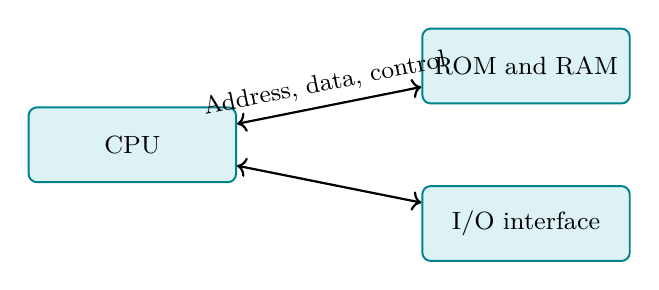
\begin{tikzpicture}
\node[block] (cpu) at (0,0) {CPU};
\node[block] (mem) at (5,1) {ROM and RAM};
\node[block] (io) at (5,-1) {I/O interface};
\draw[<->,thick] (cpu) -- (mem) node[midway,above,sloped,font=\small] {Address, data, control};
\draw[<->,thick] (cpu) -- (io);
\end{tikzpicture}
\end{tcolorbox}
\par\addvspace{7pt}\noindent
The address bus selects a byte or peripheral register, the bidirectional data bus carries its contents, and control signals identify the transfer and its timing. A decoder generates chip select from high address bits. ROM holds the reset program, while RAM holds variables and the stack. An instruction cycle can contain several bus cycles, each of which takes several clock periods (T-states). A wait state gives slower hardware extra time.

\section{Intel 8085 Architecture and Pin Description}
\begin{tcolorbox}[defbox,title={8085 Programmer's Model}]
The \href{https://www.bitsavers.org/components/intel/MCS80/9800301D_8080_8085_Assembly_Language_Programming_Manual_May81.pdf}{8085} is an 8-bit processor with a 16-bit byte address and a 64 KiB memory space. The accumulator A feeds the arithmetic and logic unit. B, C, D, E, H and L form the register pairs BC, DE and HL. PC points to the next instruction and SP points to the top of a downward-growing stack. The status flags are sign (S), zero (Z), auxiliary carry (AC), parity (P) and carry (CY).
\end{tcolorbox}
\par\addvspace{5pt}
\begingroup
\setlength{\extrarowheight}{2.5pt}
\noindent\begin{tabularx}{\linewidth}{|B{3.1cm}|Y|Y|}
\hline
\textbf{Pins} & \textbf{Signal} & \textbf{Purpose} \\ \hline
1--3 & X1, X2, RESET OUT & Clock oscillator and system reset indication. \\ \hline
4--5 & SOD, SID & Serial data output and input, used with SIM and RIM. \\ \hline
6--11 & TRAP, RST 7.5, RST 6.5, RST 5.5, INTR, $\overline{\mathrm{INTA}}$ & Interrupt requests and active-low INTR acknowledge. \\ \hline
12--19, 21--28 & AD0--AD7, A8--A15 & Multiplexed low address/data byte and dedicated high address. Pin 20 is ground. \\ \hline
29--34 & S0, ALE, $\overline{\mathrm{WR}}$, $\overline{\mathrm{RD}}$, S1, IO/M & Bus status, latch enable, read/write strobes and memory/I/O selection. \\ \hline
35--40 & READY, $\overline{\mathrm{RESET\ IN}}$, CLK OUT, HLDA, HOLD, VCC & Wait-state input, CPU reset, clock output, DMA handshake and supply. \\ \hline
\end{tabularx}\par
\endgroup
\par\addvspace{8pt}
\begin{tcolorbox}[tikzbox,unbreakable,title={8085 40-Pin DIP, Top View}]
\centering
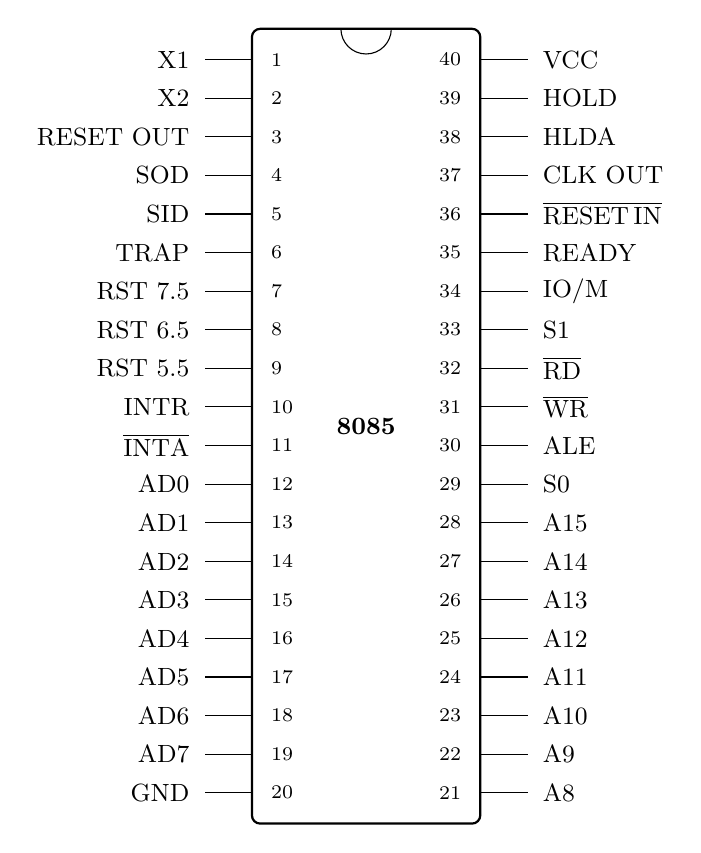
\begin{tikzpicture}[x=1cm,y=0.49cm,every node/.style={font=\small}]
\draw[thick,rounded corners=3pt] (-1.45,0.8) rectangle (1.45,-19.8);
\draw (-0.32,0.8) arc[start angle=180,end angle=360,radius=0.32cm];
\node[font=\small\bfseries] at (0,-9.5) {8085};
\foreach \i/\leftpin/\rightpin in {
{0}/{X1}/{VCC},
{1}/{X2}/{HOLD},
{2}/{RESET OUT}/{HLDA},
{3}/{SOD}/{CLK OUT},
{4}/{SID}/{$\overline{\mathrm{RESET\,IN}}$},
{5}/{TRAP}/{READY},
{6}/{RST 7.5}/{IO/M},
{7}/{RST 6.5}/{S1},
{8}/{RST 5.5}/{$\overline{\mathrm{RD}}$},
{9}/{INTR}/{$\overline{\mathrm{WR}}$},
{10}/{$\overline{\mathrm{INTA}}$}/{ALE},
{11}/{AD0}/{S0},
{12}/{AD1}/{A15},
{13}/{AD2}/{A14},
{14}/{AD3}/{A13},
{15}/{AD4}/{A12},
{16}/{AD5}/{A11},
{17}/{AD6}/{A10},
{18}/{AD7}/{A9},
{19}/{GND}/{A8}
} {
  \pgfmathtruncatemacro{\lp}{\i+1}
  \pgfmathtruncatemacro{\rp}{40-\i}
  \draw (-1.45,-\i) -- (-2.05,-\i) node[left=2pt] {\leftpin};
  \draw (1.45,-\i) -- (2.05,-\i) node[right=2pt] {\rightpin};
  \node[anchor=west,font=\scriptsize] at (-1.33,-\i) {\lp};
  \node[anchor=east,font=\scriptsize] at (1.33,-\i) {\rp};
}
\end{tikzpicture}
\par\vspace{7pt}
An overbar identifies an active-low signal. IO/M is high for I/O and low for a memory cycle.
\end{tcolorbox}

\subsection{Bus Timing and Memory Access}
In T1, AD0--AD7 carry the low address and ALE enables an external latch. The falling edge of ALE retains that address. In T2 and T3, the same pins carry data. A read cycle asserts $\overline{\mathrm{RD}}$ and the selected device drives the data bus. A write cycle asserts $\overline{\mathrm{WR}}$ and the processor drives it. A slow device can hold READY low to insert wait states. For opcode fetch, IO/M, S1 and S0 are $0,1,1$. For memory read and write the status triplets are $0,1,0$ and $0,0,1$.
\begin{tcolorbox}[examplebox,title={8085 Address Decoding}]
Map a 4 KiB ROM at \texttt{0000H} and an 8 KiB RAM at \texttt{2000H}.
\begin{enumerate}[leftmargin=*,itemsep=4pt]
\item The 4 KiB ROM needs A0--A11. Decode A15--A12 as \texttt{0000} to select \texttt{0000H--0FFFH}.
\item The 8 KiB RAM needs A0--A12. Decode A15--A13 as \texttt{001} to select \texttt{2000H--3FFFH}.
\item Use latched A0--A7 at both chips. Qualify selection for a memory cycle. Connect the read strobe to output enable and the write strobe to RAM write enable. The ROM contains the reset location \texttt{0000H}.
\end{enumerate}
\end{tcolorbox}

\section{Intel 8086 Architecture, Pins and Segmented Access}
\begin{tcolorbox}[defbox,title={Execution Unit and Bus Interface Unit}]
The \href{https://bitsavers.trailing-edge.com/components/intel/8086/9800722-03_The_8086_Family_Users_Manual_Oct79.pdf}{8086} is a 16-bit processor with a 20-bit physical byte address and a 1 MiB memory space. The \textbf{execution unit (EU)} decodes and executes instructions. The \textbf{bus interface unit (BIU)} forms addresses, manages bus cycles and prefetches up to six instruction bytes. A taken branch changes the fetch address and discards obsolete prefetched bytes.
\end{tcolorbox}
\par\addvspace{7pt}\noindent
The general registers AX, BX, CX and DX have individually accessible high and low bytes. SP and BP are stack-related registers, and SI and DI are index registers. CS:IP selects the next instruction, SS:SP selects the stack, DS usually selects data, and ES is the extra segment used as the destination segment for string operations. A BP-based effective address defaults to SS. FLAGS contains status flags CF, PF, AF, ZF, SF and OF and control flags TF, IF and DF.
\par\addvspace{6pt}
\begingroup
\setlength{\extrarowheight}{2.5pt}
\noindent\begin{tabularx}{\linewidth}{|B{2.7cm}|Y|Y|}
\hline
\textbf{DIP pins} & \textbf{Signals} & \textbf{Function} \\ \hline
1, 20, 40 & GND, GND, VCC & Supply and ground. \\ \hline
2--16, 39 & AD14--AD0, AD15 & Multiplexed low 16 address bits and data. \\ \hline
17--19, 21--23 & NMI, INTR, CLK, RESET, READY, $\overline{\mathrm{TEST}}$ & Interrupt inputs, clock, reset, wait control and input tested by WAIT. WAIT continues when TEST is low. \\ \hline
32--38 & $\overline{\mathrm{RD}}$, MN/$\overline{\mathrm{MX}}$, $\overline{\mathrm{BHE}}$/S7, A19/S6--A16/S3 & Read strobe, mode select, high-bank enable and high address/status signals. \\ \hline
24--31, minimum & $\overline{\mathrm{INTA}}$, ALE, $\overline{\mathrm{DEN}}$, DT/$\overline{\mathrm{R}}$, M/IO, $\overline{\mathrm{WR}}$, HLDA, HOLD & CPU directly supplies bus commands and HOLD/HLDA handshake. \\ \hline
24--31, maximum & QS1, QS0, S0, S1, S2, $\overline{\mathrm{LOCK}}$, $\overline{\mathrm{RQ/GT1}}$, $\overline{\mathrm{RQ/GT0}}$ & Queue and bus status, lock and arbitration. An 8288 decodes S2--S0 into bus commands. \\ \hline
\end{tabularx}\par
\endgroup
\par\addvspace{8pt}
\begin{tcolorbox}[tikzbox,unbreakable,title={8086 Minimum Mode 40-Pin DIP, Top View}]
\centering
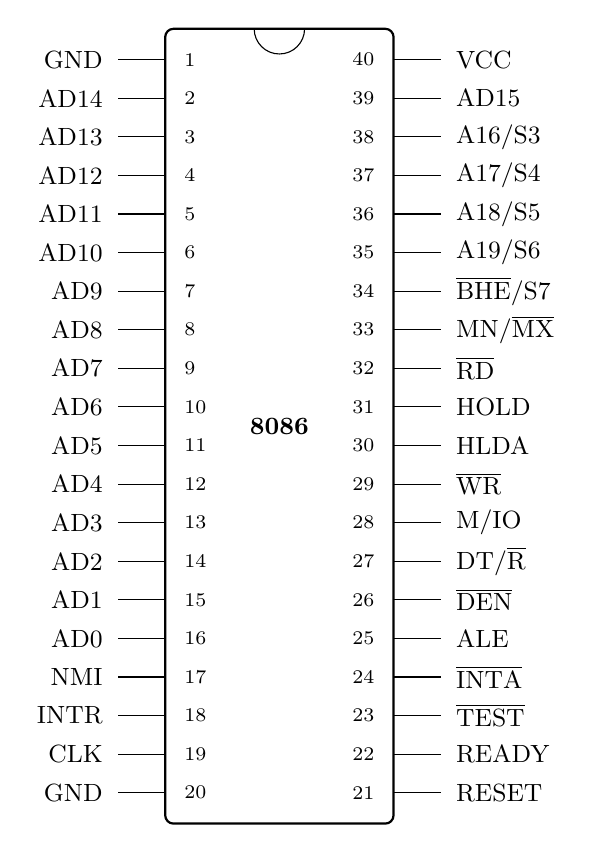
\begin{tikzpicture}[x=1cm,y=0.49cm,every node/.style={font=\small}]
\draw[thick,rounded corners=3pt] (-1.45,0.8) rectangle (1.45,-19.8);
\draw (-0.32,0.8) arc[start angle=180,end angle=360,radius=0.32cm];
\node[font=\small\bfseries] at (0,-9.5) {8086};
\foreach \i/\leftpin/\rightpin in {
{0}/{GND}/{VCC},
{1}/{AD14}/{AD15},
{2}/{AD13}/{A16/S3},
{3}/{AD12}/{A17/S4},
{4}/{AD11}/{A18/S5},
{5}/{AD10}/{A19/S6},
{6}/{AD9}/{$\overline{\mathrm{BHE}}$/S7},
{7}/{AD8}/{MN/$\overline{\mathrm{MX}}$},
{8}/{AD7}/{$\overline{\mathrm{RD}}$},
{9}/{AD6}/{HOLD},
{10}/{AD5}/{HLDA},
{11}/{AD4}/{$\overline{\mathrm{WR}}$},
{12}/{AD3}/{M/IO},
{13}/{AD2}/{DT/$\overline{\mathrm{R}}$},
{14}/{AD1}/{$\overline{\mathrm{DEN}}$},
{15}/{AD0}/{ALE},
{16}/{NMI}/{$\overline{\mathrm{INTA}}$},
{17}/{INTR}/{$\overline{\mathrm{TEST}}$},
{18}/{CLK}/{READY},
{19}/{GND}/{RESET}
} {
  \pgfmathtruncatemacro{\lp}{\i+1}
  \pgfmathtruncatemacro{\rp}{40-\i}
  \draw (-1.45,-\i) -- (-2.05,-\i) node[left=2pt] {\leftpin};
  \draw (1.45,-\i) -- (2.05,-\i) node[right=2pt] {\rightpin};
  \node[anchor=west,font=\scriptsize] at (-1.33,-\i) {\lp};
  \node[anchor=east,font=\scriptsize] at (1.33,-\i) {\rp};
}
\end{tikzpicture}
\par\vspace{7pt}
Pin 33 is held high for minimum mode. In maximum mode pins 24--31 use the alternate names listed above.
\end{tcolorbox}

\begin{tcolorbox}[formulabox,title={Segment and Offset}]
For a segment register value $S$ and a 16-bit effective offset $d$,
\[
 A_{\mathrm{physical}}=(16S+d)\bmod 2^{20}.
\]
For example, \texttt{1234H:00F0H} gives \texttt{12340H + 00F0H = 12430H}. Different segment:offset pairs can identify the same byte. A segment can cover up to 64 KiB.
\end{tcolorbox}

\subsection{Little-Endian Data and Bank Selection}
A word \texttt{1234H} is stored as byte \texttt{34H} at the lower address and byte \texttt{12H} at the next address. The even bank connects to D0--D7 and the odd bank to D8--D15. A0 selects the even bank when low, and $\overline{\mathrm{BHE}}$ selects the odd bank when low.
\par\addvspace{6pt}
\begingroup
\setlength{\extrarowheight}{2.5pt}
\noindent\begin{tabularx}{\linewidth}{|B{2.6cm}|B{2.6cm}|Y|}
\hline
\textbf{A0} & \textbf{BHE pin level} & \textbf{Transfer} \\ \hline
0 & 0 & Both banks, one aligned word transfer. \\ \hline
0 & 1 & Even byte on D0--D7. \\ \hline
1 & 0 & Odd byte on D8--D15. An odd-address word uses two cycles. \\ \hline
1 & 1 & Neither bank. \\ \hline
\end{tabularx}\par
\endgroup
In a minimum-mode system, latch AD0--AD15, the high address/status lines and bank select as needed. Route data through transceivers and use DT/$\overline{\mathrm{R}}$ and $\overline{\mathrm{DEN}}$ for direction and enable. The bus carries the address during T1, changes roles in T2, transfers data in T3, and releases the cycle in T4. Wait states can precede T4. Isolated I/O uses IN/OUT and a separate I/O address space. Memory-mapped I/O occupies memory addresses and uses normal memory instructions.

\begin{tcolorbox}[examplebox,title={8086 Boot ROM Address and Bank Design}]
Map a 32 KiB EPROM block to physical \texttt{F8000H--FFFFFH} so it contains the 8086 reset fetch at \texttt{FFFF0H}.
\begin{enumerate}[leftmargin=*,itemsep=4pt]
\item Two 16 KiB by 8 devices supply the even and odd banks. Each requires 14 chip-address bits, connected to latched CPU A1--A14.
\item Decode A19--A15 as \texttt{11111}. Within the selected block, qualify the low device using A0 low and the high device using latched BHE low.
\item Connect the devices to the low and high data bytes, respectively. Qualify output enable with the memory-read command. A reset stub in the mapped ROM jumps to the rest of the initialisation routine.
\end{enumerate}
\end{tcolorbox}

\section{Interrupts and Direct Memory Access}
\begin{tcolorbox}[defbox,title={Interrupt and DMA}]
An \textbf{interrupt} temporarily redirects the CPU to an interrupt service routine (ISR). \textbf{Direct memory access (DMA)} lets another bus master move data between memory and an interface without the CPU copying each byte.
\end{tcolorbox}
\subsection{8085 Interrupts}
\par\addvspace{5pt}
\begingroup
\setlength{\extrarowheight}{2.5pt}
\noindent\begin{tabularx}{\linewidth}{|B{2.6cm}|B{2.6cm}|Y|}
\hline
\textbf{Priority order} & \textbf{Vector} & \textbf{Recognition} \\ \hline
TRAP & \texttt{0024H} & Non-maskable, edge and level sensitive. \\ \hline
RST 7.5 & \texttt{003CH} & Maskable, rising edge latched. \\ \hline
RST 6.5 & \texttt{0034H} & Maskable, level sensitive. \\ \hline
RST 5.5 & \texttt{002CH} & Maskable, level sensitive. \\ \hline
INTR & Device supplies opcode & Maskable, level sensitive. CPU issues $\overline{\mathrm{INTA}}$. \\ \hline
\end{tabularx}\par
\endgroup
EI and DI control global maskable-interrupt acceptance. SIM controls masks for RST 7.5, 6.5 and 5.5 and can clear the RST 7.5 latch. RIM reads interrupt status and SID. The ISR saves any registers it changes, services the source, restores registers and returns with RET. Arrange interrupt re-enabling in accordance with the ISR design.
\subsection{8086 Interrupt Vector Table}
INTR is maskable through IF. NMI uses type 2 and is non-maskable. Software \texttt{INT n} selects type $n$. The 256 four-byte vectors occupy \texttt{00000H--003FFH}. Entry $4n$ holds the new IP word, followed by the new CS word. The CPU saves FLAGS, CS and IP, clears IF and TF, and jumps to the vector. IRET restores IP, CS and FLAGS. For example, type \texttt{21H} starts at \texttt{0084H}, and its CS word starts at \texttt{0086H}.

\subsection{DMA Request, Grant and Release}
\begin{tcolorbox}[tikzbox,title={Minimum-Mode DMA Handshake}]
\centering
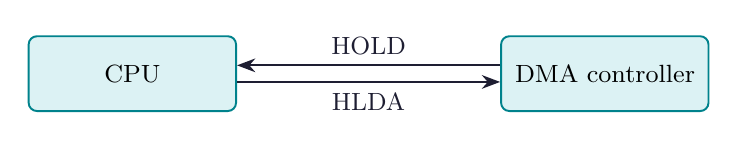
\begin{tikzpicture}
\node[block] (cpu) at (0,0) {CPU};
\node[block] (dma) at (6,0) {DMA controller};
\draw[arrow] ([yshift=3pt]dma.west) -- ([yshift=3pt]cpu.east) node[midway,above,font=\small] {HOLD};
\draw[arrow] ([yshift=-3pt]cpu.east) -- ([yshift=-3pt]dma.west) node[midway,below,font=\small] {HLDA};
\end{tikzpicture}
\end{tcolorbox}
\par\addvspace{7pt}\noindent
The device requests DMA. The controller requests the bus through HOLD. After relinquishing the bus, the CPU asserts HLDA and releases its bus outputs. The controller drives the memory address and the relevant read/write commands, updates the address and count, and releases HOLD when done. The CPU withdraws HLDA and resumes bus use. Burst transfer holds the bus for a block, while cycle stealing obtains it for individual transfers. An 8237A is an example controller. Program the start address, direction and transfer count before enabling the channel.

\subsection{Compare Polling, Interrupts and DMA}
\par\addvspace{5pt}
\begingroup
\setlength{\extrarowheight}{2.5pt}
\noindent\begin{tabularx}{\linewidth}{|B{3.1cm}|Y|Y|}
\hline
\textbf{Method} & \textbf{How it works} & \textbf{Design trade-off} \\ \hline
Polling & CPU checks a status bit repeatedly before transferring a byte. & Very simple control, but the loop uses CPU time while the device is idle. \\ \hline
Interrupts & Device signals readiness and the ISR performs the required transfer. & Good for occasional events. Entry, exit and register saving cost time. \\ \hline
DMA & A bus master carries out the data transfers after setup. & Efficient for a block. Arbitration and address/count setup add hardware complexity. \\ \hline
\end{tabularx}\par
\endgroup

\section{Instruction Sets and Assembly Examples}
An \textbf{addressing mode} specifies where an operand comes from. Register and immediate operands are internal or encoded in the instruction. A direct memory operand contains an address or offset. A register-indirect operand uses the contents of a register or pair as the address. The 8086 also supports base-plus-index and displacement combinations using permitted registers BX/BP and SI/DI.
\par\addvspace{6pt}
\begingroup
\setlength{\extrarowheight}{2.5pt}
\noindent\begin{tabularx}{\linewidth}{|B{2.8cm}|Y|Y|}
\hline
\textbf{Group} & \textbf{8085 examples} & \textbf{8086 examples} \\ \hline
Transfer and address & MOV, MVI, LXI, LDA, STA, LHLD, XCHG & MOV, LEA, XCHG, LDS, LES \\ \hline
Arithmetic & ADD, ADC, SUB, SBB, INR, DCR, DAD, DAA & ADD, ADC, SUB, SBB, INC, DEC, MUL, IMUL, DIV, IDIV \\ \hline
Logic and bit handling & ANA, ORA, XRA, CMP, RLC, RAR & AND, OR, XOR, TEST, CMP, SHL, SHR, SAR, ROL \\ \hline
Flow and stack & JMP, JZ, JC, CALL, RET, RST, PUSH, POP & JMP, JZ, JC, LOOP, CALL, RET, INT, IRET, PUSH, POP \\ \hline
I/O and control & IN, OUT, EI, DI, HLT, NOP & IN, OUT, STI, CLI, CLD, STD, HLT, WAIT \\ \hline
String operations & Explicit load, store and loop & MOVSB, LODSB, STOSB, CMPSB, SCASB with repeat prefixes as applicable. \\ \hline
\end{tabularx}\par
\endgroup

\begin{tcolorbox}[examplebox,title={Trace an 8086 Based-Indexed Access}]
For \texttt{MOV AL,[BX+SI+08H]}, let BX=\texttt{0120H}, SI=\texttt{0010H} and DS=\texttt{2000H}.
\begin{align*}
 \text{effective offset} &= \text{\texttt{0120H + 0010H + 0008H = 0138H}},\\
 \text{physical address} &= \text{\texttt{20000H + 0138H = 20138H}}.
\end{align*}
The instruction copies the selected byte into AL. Replacing BX with BP would select SS by default. Replacing the destination with AX would read a word, taking two bus cycles if the first byte started at an odd address.
\end{tcolorbox}

\subsection{Worked 8085 Addition and 8086 Block Copy}
\begin{tcolorbox}[examplebox,title={8085 Unsigned Byte Addition}]
Add the bytes at \texttt{2000H} and \texttt{2001H}, store the low byte at \texttt{2002H}, then store the carry as a byte at \texttt{2003H}. INR or DCR can change Z without altering CY. MVI and STA preserve flags here.
\end{tcolorbox}
\begin{verbatim}
        LDA  2000H
        MOV  B,A
        LDA  2001H
        ADD  B
        STA  2002H
        MVI  A,00H
        ACI  00H
        STA  2003H
        HLT
\end{verbatim}
For \texttt{F2H + 24H = 116H}, the stored bytes are \texttt{16H} and \texttt{01H}.
\begin{tcolorbox}[examplebox,title={8086 Copy Four Bytes}]
Assume DS and ES already address the source and destination segments and that the regions do not overlap. CLD makes SI and DI increment. REP repeats MOVSB until CX reaches zero. The source offset moves from \texttt{0200H} to \texttt{0204H}, and the destination from \texttt{0300H} to \texttt{0304H}.
\end{tcolorbox}
\begin{verbatim}
        CLD
        MOV  SI,0200H
        MOV  DI,0300H
        MOV  CX,4
        REP  MOVSB
\end{verbatim}
\begin{tcolorbox}[exambox,title={Exam Checks}]
In an interfacing answer, show address range, decoding, latch, control strobes and data-bus direction. For assembly, trace the registers that select operands and the flags used by decisions. A carry represents unsigned overflow. On 8086 the OF flag represents signed overflow.
\end{tcolorbox}

\newpage
\begin{center}
{\large\bfseries\color{myred} Quick Revision --- Module 1}\\[3pt]
{\small\color{mydark} 8085 and 8086 Microprocessor Systems $|$ EC403}
\end{center}
\noindent{\color{myred}\rule{\linewidth}{1.2pt}}\vspace{4pt}
\begin{tcolorbox}[formulabox,title={Key Formulas at a Glance}]
\renewcommand{\arraystretch}{1.35}
\noindent\begin{tabularx}{\linewidth}{B{4.5cm}Y}
Address capacity & $2^n$ bytes for $n$ byte-address lines. \\
Chip decoding & A $2^k$-byte chip uses $k$ internal address lines. \\
8086 address & $A_{\mathrm{physical}}=(16S+d)\bmod2^{20}$. \\
Interrupt vector & 8086 type $n$ starts at physical byte $4n$. \\
\end{tabularx}\par
\end{tcolorbox}
\begin{tcolorbox}[defbox,title={One-Line Definitions}]
\begin{itemize}[leftmargin=*,itemsep=3pt]
\item \textbf{ALE:} Address latch enable pulse used to retain a multiplexed bus address.
\item \textbf{Wait state:} Extra bus time inserted for a slower device.
\item \textbf{Vector:} A defined ISR address or a table entry that gives that address.
\item \textbf{DMA:} Data transfer managed by an alternate bus master.
\end{itemize}
\end{tcolorbox}
\begin{tcolorbox}[exambox,title={Frequently Asked / Viva Questions}]
\begin{enumerate}[leftmargin=*,label=\textbf{Q\arabic*.},itemsep=5pt]
\item \Q{What is the 8085 memory capacity?} $2^{16}$ bytes, or 64 KiB.
\item \Q{Why latch AD0--AD7?} They carry address in T1 and data later.
\item \Q{Which 8085 interrupt is non-maskable?} TRAP.
\item \Q{Which 8085 maskable interrupt is edge latched?} RST 7.5.
\item \Q{What does READY low do?} It requests a wait state while the interface becomes ready.
\item \Q{What is the 8086 prefetch queue size?} Six bytes.
\item \Q{Why does an odd-address word take two cycles?} Its bytes belong to different aligned bank pairs.
\item \Q{How is an 8086 interrupt-type entry located?} Multiply the type number by four.
\item \Q{How does the DMA controller obtain the minimum-mode bus?} It asserts HOLD and waits for HLDA.
\item \Q{How does the stack grow?} It grows towards lower addresses on both processors.
\item \Q{What does REP MOVSB modify?} It advances or retreats SI and DI according to DF and decreases CX to zero.
\end{enumerate}
\end{tcolorbox}
\begin{tcolorbox}[tikzbox,title={8085 and 8086 at a Glance}]
\par\addvspace{5pt}
\begingroup
\setlength{\extrarowheight}{2.5pt}
\noindent\begin{tabularx}{\linewidth}{|B{3.6cm}|Y|Y|}
\hline
\textbf{Feature} & \textbf{8085} & \textbf{8086} \\ \hline
Data width and memory & 8-bit, 64 KiB & 16-bit, 1 MiB \\ \hline
Addressing & 16-bit byte address & Segment:offset and even/odd banks \\ \hline
Interrupt return & RET with software register restoration & IRET restores IP, CS and FLAGS \\ \hline
\end{tabularx}\par
\endgroup
\end{tcolorbox}


% -- Module 2 -----------------------------------------------------------------
\modulestart{2}{Peripheral Interfacing and Arithmetic Coprocessors}

\section{Peripheral Interfacing and Arithmetic Coprocessors}
\begin{tcolorbox}[defbox,title={Peripheral Interface}]
A \textbf{peripheral interface} connects a CPU bus to a device with different timing, signal levels or data formats. Its data register holds the value being sent or received, its status register reports events such as ready or busy, and its control register selects how the device operates.
\end{tcolorbox}
\par\addvspace{7pt}\noindent
In an isolated I/O design the address decoder selects the interface only during an I/O cycle. In a memory-mapped design it selects the interface only during a memory cycle. The lower address lines select the internal register. In both designs, read and write strobes must meet the interface timing requirements.
\begin{tcolorbox}[tikzbox,title={Address, Control and Data Paths}]
\centering
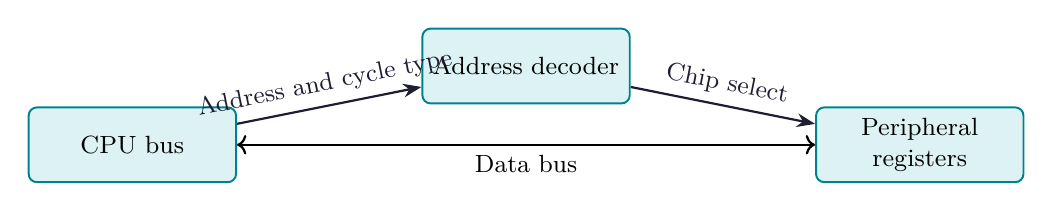
\begin{tikzpicture}
\node[block] (cpu) at (0,0) {CPU bus};
\node[block] (decode) at (5,1) {Address decoder};
\node[block] (dev) at (10,0) {Peripheral\\registers};
\draw[arrow] (cpu) -- (decode) node[midway,above,sloped,font=\small] {Address and cycle type};
\draw[arrow] (decode) -- (dev) node[midway,above,sloped,font=\small] {Chip select};
\draw[<->,thick] (cpu) -- (dev) node[midway,below,font=\small] {Data bus};
\end{tikzpicture}
\end{tcolorbox}
\par\addvspace{7pt}\noindent
Polling suits simple, low-rate transfers, but CPU time is spent reading status. Interrupt-driven I/O lets the CPU run other work until the device signals an event. DMA is useful for blocks when sustained rate matters. Handshaking keeps data valid until the receiver can accept it.

\section{Timer Interfacing with the 8253 and 8254}
\begin{tcolorbox}[defbox,title={Programmable Interval Timer}]
The 8253 and 8254 have three independent 16-bit counters. Each counts pulses at CLK, accepts control through GATE and changes its output at OUT according to the selected mode. The CPU writes a control word followed by the initial count.
\end{tcolorbox}
\par\addvspace{7pt}\noindent
A1:A0 selects counters 0, 1 and 2 or the control register at addresses 00, 01, 10 and 11. The control word selects the counter, byte-access format, mode and binary or binary-coded decimal (BCD) counting. With low-byte/high-byte access, send the low byte first. The 8254 adds a read-back command for latching count or status.
\par\addvspace{6pt}
\begingroup
\setlength{\extrarowheight}{2.5pt}
\noindent\begin{tabularx}{\linewidth}{|B{3.9cm}|Y|}
\hline
\textbf{Mode} & \textbf{Output and typical use} \\ \hline
0, terminal count & OUT goes high at completion. Delayed interrupt. \\ \hline
1, retriggerable one-shot & A GATE trigger starts a timed low pulse. \\ \hline
2, rate generator & Repeating period of $N$ clocks with a one-clock low pulse. \\ \hline
3, square-wave generator & Period of $N$ clocks. Equal high and low times for even $N$. \\ \hline
4, software-triggered strobe & Writing the count starts a delay ending in a one-clock low strobe. \\ \hline
5, hardware-triggered strobe & A rising GATE edge starts the delay. Retriggerable. \\ \hline
\end{tabularx}\par
\endgroup
\begin{tcolorbox}[examplebox,title={Design a 1 kHz Square Wave}]
Use counter 0 in mode 3 with a 1 MHz input clock and GATE high.
\begin{align*}
 N &= \frac{f_{\mathrm{CLK}}}{f_{\mathrm{OUT}}}\\
   &= \frac{10^6}{10^3}=1000=\text{\texttt{03E8H}}.
\end{align*}
The control bits are \texttt{00 11 011 0}, giving \texttt{36H}. Write \texttt{36H} to the control port, then \texttt{E8H} and \texttt{03H} to counter 0. In binary mode a count word of zero represents 65,536.
\end{tcolorbox}

\section{Parallel I/O with the 8255A}
\begin{tcolorbox}[defbox,title={Programmable Peripheral Interface}]
The 8255A provides 24 parallel I/O lines as Ports A, B and C. Port C is divided into two four-bit halves. A1:A0 selects A, B, C or the control register in order. RESET places the ports in input configuration.
\end{tcolorbox}
\par\addvspace{6pt}
\begingroup
\setlength{\extrarowheight}{2.5pt}
\noindent\begin{tabularx}{\linewidth}{|B{3cm}|Y|}
\hline
\textbf{Mode} & \textbf{Operation} \\ \hline
0 & Basic parallel I/O. Outputs are latched. Inputs can be sampled directly. \\ \hline
1 & Strobed input or output on Port A or B. Selected Port C lines provide handshaking and interrupt signals. \\ \hline
2 & Bidirectional strobed data on Port A. Its handshaking uses Port C lines. Port B can use mode 0 or 1. \\ \hline
BSR & Bit set/reset changes an individual Port C latch bit. Control word D7 is zero. \\ \hline
\end{tabularx}\par
\endgroup
In a mode 1 input transaction, the peripheral asserts STB to latch data, the interface reports input-buffer full (IBF), and the CPU reads the port. On output the CPU writes a byte, output-buffer full (OBF) signals the device, and ACK confirms acceptance. INTR can signal the CPU when the corresponding interrupt enable is set.
\begin{tcolorbox}[examplebox,title={Switches on Port B and LEDs on Port A}]
Choose mode 0, A output, B input and both halves of C output. In the mode-set word D7=1, D6:D5=00, D4=0, D3=0, D2=0, D1=1 and D0=0, so write \texttt{82H} to the control port. Read B, then write the byte to A. Use suitable resistors and a driver where the LED current exceeds the port rating. For BSR, D3:D1 encode the Port C bit number and D0 selects set (1) or reset (0). The words \texttt{0BH} and \texttt{0AH} set and reset PC5.
\end{tcolorbox}

\subsection{8255A Mode 1 Port C Signals}
\par\addvspace{5pt}
\begingroup
\setlength{\extrarowheight}{2.5pt}
\noindent\begin{tabularx}{\linewidth}{|B{3.2cm}|Y|Y|}
\hline
\textbf{Mode 1 group} & \textbf{Input signalling} & \textbf{Output signalling} \\ \hline
Port A & PC4 is STB, PC5 is IBF, and PC3 is INTR. & PC7 is OBF, PC6 is ACK, and PC3 is INTR. \\ \hline
Port B & PC2 is STB, PC1 is IBF, and PC0 is INTR. & PC1 is OBF, PC2 is ACK, and PC0 is INTR. \\ \hline
\end{tabularx}\par
\endgroup
STB, OBF and ACK are active-low signals. The mode determines which Port C bits are assigned to the handshake. Treat these pins as signals for that handshake while the mode is active.

\section{Serial I/O with the 8251A}
\begin{tcolorbox}[defbox,title={USART and Serial Framing}]
A \textbf{universal synchronous/asynchronous receiver/transmitter (USART)} converts parallel CPU data into a serial bit stream and converts received bits back into parallel data. Asynchronous framing adds a start bit and stop bit or bits to each character. Synchronous operation uses a shared bit clock and synchronisation characters.
\end{tcolorbox}
\par\addvspace{7pt}\noindent
The CPU selects data or control/status using C/D. After reset, write the mode instruction defining the character format and clock factor. In synchronous mode write the required sync characters, then write a command to enable the transmitter or receiver. On transmission, test TxRDY before writing each character. On reception, test RxRDY, read the byte, and handle parity, overrun and framing errors. TxEMPTY indicates the transmitter buffer and shift path are empty, which matters before disabling a line driver. TXC and RXC provide transmit and receive clocks. TXD and RXD are logic-level data pins, so use an appropriate transceiver for RS-232.
\begin{tcolorbox}[examplebox,title={9600 Baud and an 8N1 Character}]
For asynchronous 16-times operation, the clock is
\[
 f_{\mathrm{clock}}=16(9600)=153.6\ \mathrm{kHz}.
\]
Eight data bits, no parity and one stop bit give mode word \texttt{4EH} for the 8251A at the 16-times setting. The link sends one start bit, eight data bits and one stop bit. With no gaps the payload rate is $9600/10=960$ characters/s.
\end{tcolorbox}

\subsection{Transmit and Receive a Byte}
Write the mode word after hardware reset, then set TxEN and RxE in the command word. Ensure CTS is at its asserted level when transmission is required. To send one byte, check TxRDY, write the data register and let the USART add the framing bits. To receive, check RxRDY, read the data register and check or handle the error flags using the command register as required. An overrun means a new character arrived before the preceding one was read. It is a service-rate problem, while a framing error usually indicates a wrong stop-bit level, clock mismatch or line problem.

\section{Analog-to-Digital and Digital-to-Analog Interfaces}
\begin{tcolorbox}[defbox,title={ADC, DAC and Resolution}]
An \textbf{analog-to-digital converter (ADC)} assigns a digital code to an analog input range. A \textbf{digital-to-analog converter (DAC)} converts a digital code to a voltage or current. An ideal $n$-bit converter has $2^n$ codes, and for a specified span $V_{\mathrm{span}}$ the ideal code step is $V_{\mathrm{span}}/2^n$.
\end{tcolorbox}
\begin{tcolorbox}[tikzbox,title={Acquisition and Analog Output Paths}]
\centering
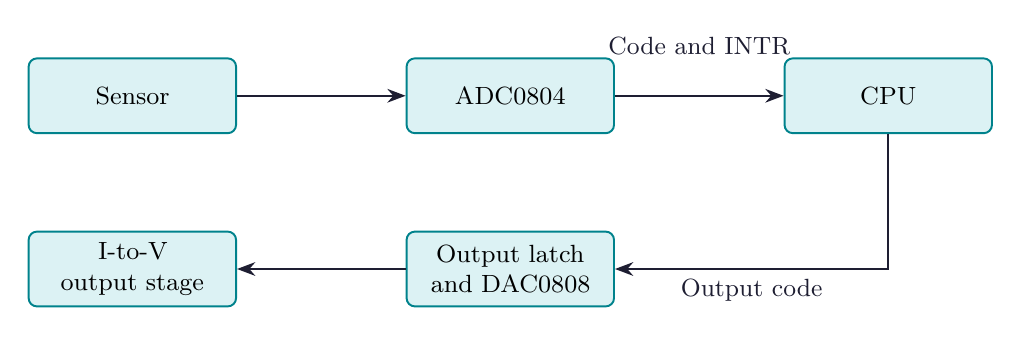
\begin{tikzpicture}
\node[block] (sensor) at (0,1.2) {Sensor};
\node[block] (adc) at (4.8,1.2) {ADC0804};
\node[block] (cpu) at (9.6,1.2) {CPU};
\node[block] (dac) at (4.8,-1.0) {Output latch\\and DAC0808};
\node[block] (out) at (0,-1.0) {I-to-V\\output stage};
\draw[arrow] (sensor) -- (adc);
\draw[arrow] (adc) -- (cpu) node[midway,above=11pt,font=\small] {Code and INTR};
\draw[arrow] (cpu.south) |- (dac.east) node[pos=.75,below,font=\small] {Output code};
\draw[arrow] (dac) -- (out);
\end{tikzpicture}
\end{tcolorbox}
\subsection{ADC0804 Successive-Approximation Interface}
A successive-approximation converter compares the input with trial values, starting at the most significant bit (MSB). The ADC0804 uses differential inputs, an external or RC clock and active-low CS, WR and RD. With CS low, pulse WR low and release it to start conversion. Wait until INTR falls, then assert RD low to read the tri-state 8-bit result. Use a stable input during conversion, and choose the reference and analog grounding for the required input range. The VREF/2 pin sets half the differential full-scale span when driven.
\begin{tcolorbox}[examplebox,title={Resolution and Example Code}]
For an ideal 8-bit converter over 0--5 V, $\Delta=5/256=19.53\ \mathrm{mV}$. An input of 2.5 V is at half scale, about code \texttt{80H}. Under an ideal rounding model, the interior quantisation uncertainty is $\pm\Delta/2$. The actual code near a boundary depends on the transfer characteristic and practical errors.
\end{tcolorbox}
\subsection{DAC0808 Current Output}
The DAC0808 uses a reference current and digital input bits to produce an output current. A latch holds the CPU's 8-bit word. An op-amp current-to-voltage stage can convert the DAC current into a voltage, with the sign and scale set by the circuit.
\begin{tcolorbox}[examplebox,title={DAC Code and Current}]
For unsigned code $D$ in an ideal 8-bit model,
\[
 I_{\mathrm{out}}=I_{\mathrm{ref}}\frac{D}{256}.
\]
For \texttt{C0H}, $D=192$ and $I_{\mathrm{out}}=1.50\ \mathrm{mA}$ when $I_{\mathrm{ref}}=2.00\ \mathrm{mA}$. For an ideal inverting converter, a $2\ \mathrm{k}\Omega$ feedback resistor gives $-3.00\ \mathrm{V}$. The highest code is 255, so the current is one step below the reference current.
\end{tcolorbox}

\section{Arithmetic Coprocessors and System-Level Design}
\begin{tcolorbox}[defbox,title={8087 Numeric Coprocessor}]
A \textbf{coprocessor} executes a specialised group of operations under coordination with the main processor. The Intel 8087 adds floating-point arithmetic to an 8086/8088 system and uses a stack of eight 80-bit extended-precision registers. It supports operations such as load, add, multiply, divide and square root.
\end{tcolorbox}
\par\addvspace{7pt}\noindent
The 8087 works with the CPU in a maximum-mode system. It monitors the instruction stream and queue status, recognises numeric ESC instructions and acquires the bus when required to transfer operands. The CPU forms effective addresses for memory operands. The 8087 BUSY signal connects to the CPU's TEST input. WAIT/FWAIT synchronises the CPU before depending on a coprocessor result. Large parts of the CPU program can continue independently where no result is needed yet.
\begin{tcolorbox}[examplebox,title={Integrated 8085 Data Acquisition and Output}, title after break={Data Acquisition and Output (contd.)}]
Use isolated I/O. Decode A7--A2 for each four-port block and feed A1:A0 to each 8255A and 8253.
\par\addvspace{6pt}
\begingroup
\setlength{\extrarowheight}{2.5pt}
\noindent\begin{tabularx}{\linewidth}{|B{3cm}|Y|}
\hline
\textbf{I/O ports} & \textbf{Assignment} \\ \hline
\texttt{40H--43H} & 8255A ports A, B, C and control. \\ \hline
\texttt{48H--4BH} & Timer counters 0, 1, 2 and control. \\ \hline
\texttt{50H}, \texttt{51H} & 8251A data and control/status. Decode A0 as C/D. \\ \hline
\texttt{58H} & ADC command on a write, conversion byte on a read. Route INTR to status or to an interrupt input with suitable polarity/timing conditioning. \\ \hline
\texttt{60H} & DAC input latch on a write. \\ \hline
\end{tabularx}\par
\endgroup
The timer signals the sample interval. Firmware starts the ADC, waits for completion, reads the byte and writes it to the DAC latch. Verify that conversion and service time fit the sampling period. Only one read device may drive the data bus at a time. Decode all relevant address bits to prevent aliases, or document any intentional aliases. Check propagation delay, setup and hold times, input levels, grounding and interrupt polarity.
\end{tcolorbox}
\par\addvspace{7pt}\noindent
For an 8086 interface on D0--D7, use even port addresses and qualify selection for the lower byte bank. Wire CPU A1, A2 to peripheral A0, A1 when four consecutive peripheral registers map to ports two apart.

\subsection*{References}
Intel's \textit{Microprocessor and Peripheral Handbook}, the \href{https://www.ti.com/lit/ds/symlink/adc0804-n.pdf}{TI ADC080x data sheet}, and the \href{https://www.ti.com/lit/ds/symlink/dac0808.pdf}{TI DAC0808 data sheet} describe the device signals and timing.

\newpage
\begin{center}
{\large\bfseries\color{myred} Quick Revision --- Module 2}\\[3pt]
{\small\color{mydark} Peripheral Interfacing and Coprocessors $|$ EC403}
\end{center}
\noindent{\color{myred}\rule{\linewidth}{1.2pt}}\vspace{4pt}
\begin{tcolorbox}[formulabox,title={Key Formulas at a Glance}]
\renewcommand{\arraystretch}{1.35}
\noindent\begin{tabularx}{\linewidth}{B{4.2cm}Y}
Timer period & $T=N/f_{\mathrm{CLK}}$ in modes 2 and 3. \\
USART clock & $f_{\mathrm{clock}}=kR$ with the selected async factor $k$ and baud rate $R$. \\
ADC step & $\Delta=V_{\mathrm{span}}/2^n$. \\
DAC output & $I_{\mathrm{out}}=I_{\mathrm{ref}}D/2^8$ for the DAC0808 model. \\
\end{tabularx}\par
\end{tcolorbox}
\begin{tcolorbox}[defbox,title={One-Line Definitions}]
\begin{itemize}[leftmargin=*,itemsep=3pt]
\item \textbf{Chip select:} Signal that enables one device to respond to a bus cycle.
\item \textbf{Handshaking:} Exchange of data-ready and acknowledgement signals.
\item \textbf{Baud:} Number of signalling symbols sent per second.
\item \textbf{Quantisation:} Assignment of an analog level to one of a finite number of codes.
\end{itemize}
\end{tcolorbox}
\begin{tcolorbox}[exambox,title={Frequently Asked / Viva Questions}]
\begin{enumerate}[leftmargin=*,label=\textbf{Q\arabic*.},itemsep=5pt]
\item \Q{What are the three timer signals?} CLK, GATE and OUT.
\item \Q{Which timer mode generates a square wave?} Mode 3.
\item \Q{How many data lines does an 8255A provide?} 24, arranged as three eight-bit ports.
\item \Q{What makes 8255 mode 2 different?} Port A transfers data in either direction using handshaking.
\item \Q{What does BSR change?} One selected Port C latch bit.
\item \Q{What marks the start of an async character?} The start bit.
\item \Q{What does RxRDY report?} A received character is available to read.
\item \Q{How does the ADC0804 indicate completion?} INTR goes low.
\item \Q{What kind of output comes from the DAC0808?} Current.
\item \Q{Why does the 8087 use WAIT?} WAIT lets the CPU synchronise with BUSY before it needs the result.
\item \Q{Why decode every relevant address bit?} It prevents unwanted mirrored addresses and bus contention.
\end{enumerate}
\end{tcolorbox}
\begin{tcolorbox}[tikzbox,title={Peripheral Selection at a Glance}]
\par\addvspace{5pt}
\begingroup
\setlength{\extrarowheight}{2.5pt}
\noindent\begin{tabularx}{\linewidth}{|B{3.2cm}|Y|Y|}
\hline
\textbf{Device} & \textbf{Function} & \textbf{Check before transfer} \\ \hline
8253/8254 & Timing or pulse generation & Mode, count, clock, gate. \\ \hline
8255A & Parallel data & Port direction and handshake. \\ \hline
8251A & Serial data & Frame format, clock, ready status. \\ \hline
ADC/DAC & Analog conversion & Scaling, completion or latch timing. \\ \hline
\end{tabularx}\par
\endgroup
\end{tcolorbox}


% -- Module 3 -----------------------------------------------------------------
\modulestart{3}{Memory Hierarchy, x86 Evolution and 8051}

\section{Memory Hierarchy, x86 Evolution and 8051}
\subsection{Virtual Address Space and Paging}
\begin{tcolorbox}[defbox,title={Virtual Address Space}]
\textbf{Virtual memory} gives each process its own view of memory. The processor generates a virtual address, which the memory management unit (MMU) translates to a physical address. Translation allows isolation, controlled sharing and keeping only the currently needed parts of an address space in RAM.
\end{tcolorbox}
\par\addvspace{7pt}\noindent
A \textbf{page} is a fixed-size virtual block. A \textbf{frame} is an equally sized physical block. A page-table entry identifies the frame when present and records access permissions. Hardware may also track whether a page was accessed or written. The page offset is the position within a page and is unchanged by translation.
\begin{tcolorbox}[tikzbox,title={Paged Address Translation}]
\centering
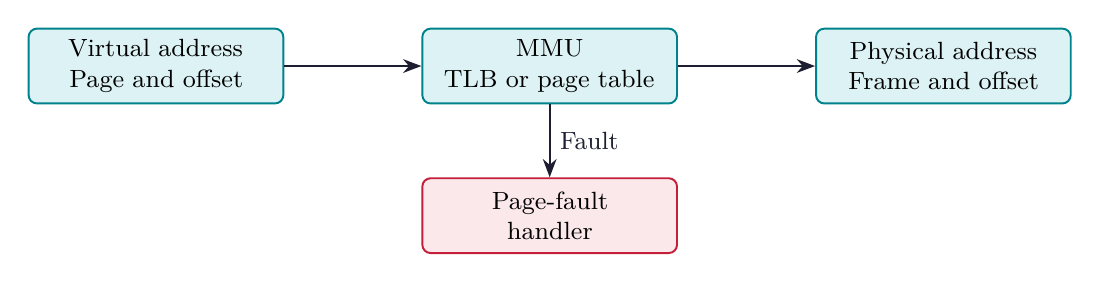
\begin{tikzpicture}
\node[block,text width=3cm] (v) at (0,0) {Virtual address\\Page and offset};
\node[block,text width=3cm] (m) at (5,0) {MMU\\TLB or page table};
\node[block,text width=3cm] (p) at (10,0) {Physical address\\Frame and offset};
\draw[arrow] (v) -- (m);
\draw[arrow] (m) -- (p);
\node[redblock,text width=3cm] (f) at (5,-1.9) {Page-fault\\handler};
\draw[arrow] (m) -- (f) node[midway,right,font=\small] {Fault};
\end{tikzpicture}
\end{tcolorbox}
\par\addvspace{7pt}\noindent
The \textbf{translation lookaside buffer (TLB)} caches translations. A TLB hit can avoid a page-table walk. On a TLB miss, hardware or software searches the page table. A present and permitted page can refill the TLB without disk access. A page fault transfers control to the operating system. An invalid access may be rejected. A valid demand-paged access can allocate a frame, evict a victim if needed, write it back if dirty and backed by writable storage, load or create the requested page, update translation state, and restart the instruction.
\begin{tcolorbox}[examplebox,title={Translate a Virtual Address}]
With 4 KiB pages and virtual address \texttt{12345H},
\begin{align*}
 \text{page size} &= 4096=2^{12}\ \text{bytes},\\
 \text{virtual page} &= \text{\texttt{12H}},\qquad
 \text{offset} = \text{\texttt{345H}}.
\end{align*}
If the page maps to frame \texttt{2AH}, the physical address is \texttt{2A000H + 345H = 2A345H}. A TLB miss alone does not imply a page fault.
\end{tcolorbox}
\subsection{Paging, Segmentation and Replacement}
\textbf{Segmentation} uses variable-size logical regions. A selector identifies a descriptor with base, limit and permissions. Adding the offset to the base gives the linear address when checks pass. Segmentation can leave external holes. Paging uses fixed-size frames and can leave unused space in the last page of an allocation. The two mechanisms can coexist.
When no frame is free, FIFO evicts the oldest resident page and least recently used (LRU) favours a page that has not recently been referenced. Clock is an approximation based on an accessed bit. If active pages are repeatedly evicted and needed again, the system can spend much of its time handling faults. This is \textbf{thrashing}.

\section{Cache Memory}
\begin{tcolorbox}[defbox,title={Cache, Hit and Miss}]
A \textbf{cache} holds copies of recently or nearby accessed memory blocks in fast storage. A \textbf{hit} finds the requested block in the cache. A \textbf{miss} fetches it from a lower level. Temporal locality means recently used data is likely to be reused. Spatial locality means nearby data is likely to be accessed soon.
\end{tcolorbox}
\par\addvspace{7pt}\noindent
Each cache line stores a block, a tag and a valid bit. A write-back cache also tracks whether the line is dirty. The address offset selects a byte within a block. The index selects a set, and the tag distinguishes memory blocks that use that set.
\par\addvspace{6pt}
\begingroup
\setlength{\extrarowheight}{2.5pt}
\noindent\begin{tabularx}{\linewidth}{|B{3.5cm}|Y|Y|}
\hline
\textbf{Mapping} & \textbf{Placement} & \textbf{Trade-off} \\ \hline
Direct mapped & One location for each block. & Fast lookup, more conflict misses. \\ \hline
Fully associative & Any line is eligible. & Fewer placement conflicts, more tag comparisons. \\ \hline
Set associative & Any of $W$ lines in one indexed set. & Balances comparison hardware and flexibility. \\ \hline
\end{tabularx}\par
\endgroup
\subsection{Write Policies and Misses}
\textbf{Write-through} updates the lower level when the cache is written, often through a write buffer. \textbf{Write-back} updates the cache and writes dirty blocks to the lower level when required, for example on eviction. \textbf{Write-allocate} fetches a line after a write miss, while \textbf{no-write-allocate} sends that write to the lower level without allocating the line. These are separate design decisions.
First-use misses are compulsory. Capacity misses arise when the cache is too small for the active blocks. Conflict misses arise when multiple blocks compete for the same set. In an associative set, LRU, approximate LRU or another policy chooses the victim if every way is occupied.
\begin{tcolorbox}[examplebox,title={Cache Address Fields and Average Access Time}]
For 32-bit byte addresses, a 16 KiB, four-way cache with 32-byte lines has
\begin{align*}
 \text{sets} &= 16384/(4\cdot32)=128,\\
 \text{offset bits} &= \log_2 32=5,\\
 \text{index bits} &= \log_2 128=7,\\
 \text{tag bits} &=32-5-7=20.
\end{align*}
If the hit time is 2 ns, the miss rate is 5\% and the \emph{additional} miss penalty is 40 ns, the average memory access time is $2+0.05(40)=4$ ns.
\end{tcolorbox}

\begin{tcolorbox}[examplebox,title={Identify Two Blocks That Conflict}]
A direct-mapped cache has eight lines and four bytes per block. For byte address $a$, the memory block number is $\lfloor a/4\rfloor$, and the line index is the block number modulo eight.
\begin{align*}
 a=4 &: \quad \text{block }1,\ \text{line }1,\ \text{tag }0,\\
 a=36 &: \quad \text{block }9,\ \text{line }1,\ \text{tag }1.
\end{align*}
With an empty cache, accesses to $4,36,4$ all miss. The third miss happens because the second access replaced the first block, even though other lines were free. The same blocks could coexist in a two-way set with two available ways.
\end{tcolorbox}

\section{80286, 80486 and Pentium Architectures}
The syllabus groups these under advanced coprocessor architectures. The 80286, 80486 and Pentium are main x86 processors. The comparison tracks how memory management and numeric coprocessor functions evolved.
\subsection{80286 Protected Mode and 80287}
The 80286 has a 16-bit data bus and a 24-bit physical address bus, giving up to 16 MiB of physical memory in protected mode. Real-address mode supports the 8086-style environment. Protected mode uses segment descriptors, access checks and four privilege levels. Selectors locate descriptors in the global or local descriptor table. Descriptors record the segment base, limit and access rights. The 80286 provides segment-based virtual memory support without hardware paging. The optional 80287 performs x87 floating-point operations.
\subsection{80486 Integration}
The original i486DX uses a 32-bit data bus, a 32-bit physical address space and a scalar instruction pipeline. It integrates an 8 KiB unified L1 cache, x87 floating-point unit (FPU), segmentation and hardware paging. A unified cache shares capacity between instructions and data. The 486SX variant does not provide a usable on-chip FPU. These details refer to the original models, since later 486 parts varied.
\subsection{Original Pentium Superscalar Execution}
A \textbf{superscalar} processor can issue more than one instruction in a cycle when the instructions can execute together. The original Pentium uses U and V integer pipelines. The U pipe accepts the broader instruction set, while the V pipe accepts eligible simple instructions in supported pairs. A data dependency or a pairing restriction can prevent dual issue. The processor adds dynamic branch prediction, separate 8 KiB instruction and 8 KiB data L1 caches, integrated floating-point hardware, a 64-bit external data bus and 32-bit physical addressing. The external data bus width is distinct from operand and address width.
\par\addvspace{6pt}
\begingroup
\setlength{\extrarowheight}{2.5pt}
\noindent\begin{tabularx}{\linewidth}{|B{3.0cm}|Y|Y|Y|}
\hline
\textbf{Feature} & \textbf{80286} & \textbf{i486DX} & \textbf{Original Pentium} \\ \hline
External data bus & 16 bits & 32 bits & 64 bits \\ \hline
Physical address bits & 24 & 32 & 32 \\ \hline
Protected memory & Segmentation & Segmentation and paging & Segmentation and paging \\ \hline
On-chip L1 & No & 8 KiB unified & 8 KiB I + 8 KiB D \\ \hline
Numeric unit & Optional 80287 & Integrated x87 & Integrated x87 \\ \hline
\end{tabularx}\par
\endgroup

\section{Classic 8051 System, Pinout and Ports}
\begin{tcolorbox}[defbox,title={Classic 8051 Microcontroller}]
The original Intel 8051 is an 8-bit microcontroller with 4 KiB on-chip program ROM, 128 bytes of internal RAM, 32 I/O lines, two 16-bit timers, a serial port and five interrupt sources. It has separate code and data address spaces. Its accumulator A processes byte data, B assists multiply and divide, PSW contains flags and register-bank selection, DPTR is a 16-bit pointer, and PC and SP control instruction and stack access.
\end{tcolorbox}
\par\addvspace{8pt}
\begin{tcolorbox}[tikzbox,unbreakable,title={Classic 8051 40-Pin DIP, Top View}]
\centering
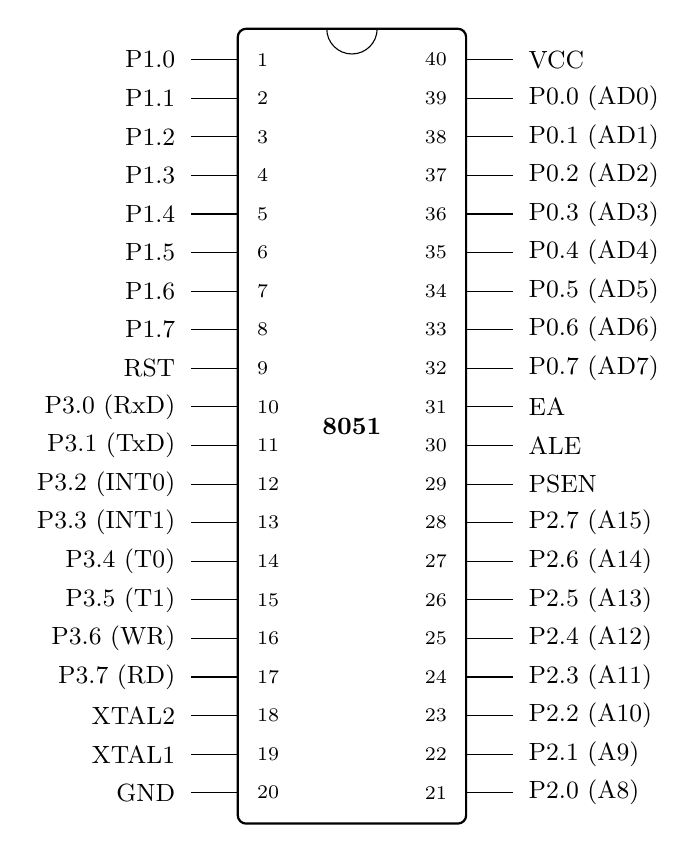
\begin{tikzpicture}[x=1cm,y=0.49cm,every node/.style={font=\small}]
\draw[thick,rounded corners=3pt] (-1.45,0.8) rectangle (1.45,-19.8);
\draw (-0.32,0.8) arc[start angle=180,end angle=360,radius=0.32cm];
\node[font=\small\bfseries] at (0,-9.5) {8051};
\foreach \i/\leftpin/\rightpin in {
0/P1.0/VCC,1/P1.1/P0.0 (AD0),2/P1.2/P0.1 (AD1),3/P1.3/P0.2 (AD2),
4/P1.4/P0.3 (AD3),5/P1.5/P0.4 (AD4),6/P1.6/P0.5 (AD5),7/P1.7/P0.6 (AD6),
8/RST/P0.7 (AD7),9/P3.0 (RxD)/EA,10/P3.1 (TxD)/ALE,11/P3.2 (INT0)/PSEN,
12/P3.3 (INT1)/P2.7 (A15),13/P3.4 (T0)/P2.6 (A14),14/P3.5 (T1)/P2.5 (A13),
15/P3.6 (WR)/P2.4 (A12),16/P3.7 (RD)/P2.3 (A11),17/XTAL2/P2.2 (A10),
18/XTAL1/P2.1 (A9),19/GND/P2.0 (A8)} {
  \pgfmathtruncatemacro{\lp}{\i+1}
  \pgfmathtruncatemacro{\rp}{40-\i}
  \draw (-1.45,-\i) -- (-2.05,-\i) node[left=2pt] {\leftpin};
  \draw (1.45,-\i) -- (2.05,-\i) node[right=2pt] {\rightpin};
  \node[anchor=west,font=\scriptsize] at (-1.33,-\i) {\lp};
  \node[anchor=east,font=\scriptsize] at (1.33,-\i) {\rp};
}
\end{tikzpicture}
\par\vspace{7pt}
EA, PSEN, INT0, INT1, WR and RD are active low. The drawing uses pin names without overbars for readability.
\end{tcolorbox}

\begin{tcolorbox}[tikzbox,title={8051 System Building Blocks}]
\centering
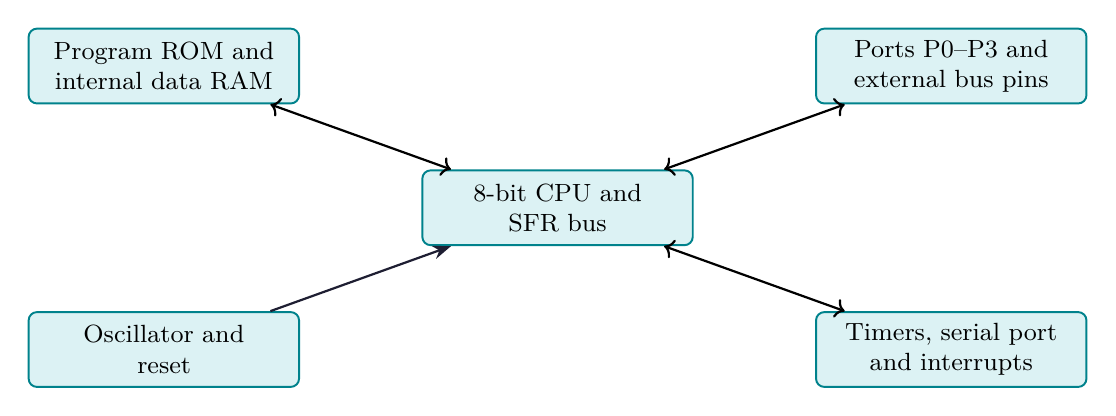
\begin{tikzpicture}
\node[block,text width=3.2cm] (core) at (0,0) {8-bit CPU and\\SFR bus};
\node[block,text width=3.2cm] (mem) at (-5,1.8) {Program ROM and\\internal data RAM};
\node[block,text width=3.2cm] (ports) at (5,1.8) {Ports P0--P3 and\\external bus pins};
\node[block,text width=3.2cm] (clock) at (-5,-1.8) {Oscillator and\\reset};
\node[block,text width=3.2cm] (peri) at (5,-1.8) {Timers, serial port\\and interrupts};
\draw[<->,thick] (core) -- (mem);
\draw[<->,thick] (core) -- (ports);
\draw[arrow] (clock) -- (core);
\draw[<->,thick] (core) -- (peri);
\end{tikzpicture}
\end{tcolorbox}
\subsection{Pin and Port Roles}
\par\addvspace{5pt}
\begingroup
\setlength{\extrarowheight}{2.5pt}
\noindent\begin{tabularx}{\linewidth}{|B{2.6cm}|B{2.4cm}|Y|}
\hline
\textbf{Signals} & \textbf{Pins} & \textbf{Uses and electrical behaviour} \\ \hline
P0 & 32--39 & AD7--AD0 in external bus cycles. In ordinary GPIO use it is open drain, so add pull-ups for a driven high level. \\ \hline
P1 & 1--8 & General-purpose quasi-bidirectional I/O with internal pull-ups on the original 8051. \\ \hline
P2 & 21--28 & GPIO or A8--A15 for external code fetch and 16-bit external-data addressing. \\ \hline
P3 & 10--17 & GPIO with internal pull-ups and eight alternate functions. \\ \hline
RST, XTAL1/2 & 9, 19/18 & Active-high reset and oscillator connections. On the classic core hold RST high for at least two machine cycles with the oscillator running. \\ \hline
PSEN, ALE, EA & 29--31 & External code read, low-address latch pulse and program-memory selection. \\ \hline
GND, VCC & 20, 40 & Ground and supply. \\ \hline
\end{tabularx}\par
\endgroup
Write a 1 to a quasi-bidirectional latch before reading an externally driven input. A 0 drives the line low. In ordinary P0 use a 1 releases the open-drain pin. Use the port electrical ratings or a driver when connecting LEDs, motors or other loads. Some read-modify-write instructions use the port latch to avoid accidentally rewriting the external pin state. An instruction such as \texttt{MOV A,P1} reads the pins.
\par\addvspace{6pt}
\begingroup
\setlength{\extrarowheight}{2.5pt}
\noindent\begin{tabularx}{\linewidth}{|B{2.5cm}|B{3cm}|Y|}
\hline
\textbf{Bit} & \textbf{Alternate function} & \textbf{Purpose} \\ \hline
P3.0, P3.1 & RxD, TxD & Serial receive and transmit. \\ \hline
P3.2, P3.3 & INT0, INT1 & External interrupt inputs. \\ \hline
P3.4, P3.5 & T0, T1 & Timer/counter external inputs. \\ \hline
P3.6, P3.7 & WR, RD & Active-low external data write/read strobes. \\ \hline
\end{tabularx}\par
\endgroup

\subsection{Code, Data and External Memory Cycles}
The internal RAM occupies \texttt{00H--7FH}. It includes register banks at \texttt{00H--1FH}, bit-addressable RAM at \texttt{20H--2FH}, and general-purpose RAM above that. Direct addresses \texttt{80H--FFH} refer to special-function registers (SFRs) where implemented. P0, P1, P2 and P3 latch addresses are \texttt{80H}, \texttt{90H}, \texttt{A0H} and \texttt{B0H}. The stack grows upward in internal RAM.
EA low directs code fetches externally. On the original 4 KiB ROM part, EA high enables internal code at \texttt{0000H--0FFFH} and higher code addresses are external. External code and external data each have their own 64 KiB space. PSEN reads external code. MOVC reads code bytes as data, and MOVX accesses external data. In a typical external memory interface, P0 carries A0--A7 during ALE and then data. An external latch holds the low address. P2 carries the high address for 16-bit external accesses. A MOVX instruction with an eight-bit register address uses the P2 latch value on the P2 pins for any external page selection. RD/WR qualify external data transfers.
\begin{tcolorbox}[examplebox,title={Read a Switch and Drive an LED}]
Connect an active-low switch to P1.0 and an active-low LED with a suitable driver to P1.1. Before reading the switch, set its port latch high so it can act as an input. The carry receives the sampled switch level and is copied to the LED output. A pressed switch has level 0 and turns the LED on.
\end{tcolorbox}
\begin{verbatim}
        SETB P1.0
again:  MOV  C,P1.0
        MOV  P1.1,C
        SJMP again
\end{verbatim}
Mechanical switches may need debouncing when a clean transition is required. Some compatible 8051-family parts have different timing, RAM or port options, so check the actual device before using the classic values.

\subsection*{References}
\href{https://people.csail.mit.edu/rinard/teaching/osnotes/h9.html}{MIT paging notes}. Intel manuals for the \href{https://www.bitsavers.org/components/intel/80286/210498-003_iAPX_286_Programmers_Reference_1985.pdf}{80286}, \href{https://bitsavers.org/components/intel/80486/i486_Processor_Programmers_Reference_Manual_1990.pdf}{i486}, \href{https://www.bitsavers.org/components/intel/pentium/1993_Intel_Pentium_Processor_Users_Manual_Volume_1.pdf}{Pentium}, and \href{https://www.bitsavers.org/components/intel/8051/MCS-51_Users_Manual_Feb94.pdf}{MCS-51}.

\newpage
\begin{center}
{\large\bfseries\color{myred} Quick Revision --- Module 3}\\[3pt]
{\small\color{mydark} Virtual Memory, Cache, x86 Evolution and 8051 $|$ EC403}
\end{center}
\noindent{\color{myred}\rule{\linewidth}{1.2pt}}\vspace{4pt}
\begin{tcolorbox}[formulabox,title={Key Formulas at a Glance}]
\renewcommand{\arraystretch}{1.35}
\noindent\begin{tabularx}{\linewidth}{B{4.2cm}Y}
Page translation & Physical address $=(\text{frame}\times \text{page size})+\text{offset}$. \\
Cache sets & $S=C/(BW)$ for data capacity $C$, block bytes $B$ and ways $W$. \\
Cache fields & Offset $\log_2 B$, index $\log_2 S$, remaining bits are tag. \\
Average access time & Hit time $+$ miss rate $\times$ additional miss penalty. \\
\end{tabularx}\par
\end{tcolorbox}
\begin{tcolorbox}[defbox,title={One-Line Definitions}]
\begin{itemize}[leftmargin=*,itemsep=3pt]
\item \textbf{Page fault:} An exception raised when a virtual-memory translation or access requires operating-system handling.
\item \textbf{TLB:} A cache of recent virtual-to-physical translations.
\item \textbf{Dirty line:} A cache line changed since the lower level was updated.
\item \textbf{Superscalar:} Able to issue multiple instructions in a clock cycle under suitable conditions.
\end{itemize}
\end{tcolorbox}
\begin{tcolorbox}[exambox,title={Frequently Asked / Viva Questions}]
\begin{enumerate}[leftmargin=*,label=\textbf{Q\arabic*.},itemsep=5pt]
\item \Q{What remains unchanged in paged translation?} The offset within the page.
\item \Q{Can a TLB miss be serviced without a page fault?} Yes. A valid page-table entry can refill the TLB.
\item \Q{What causes a cache conflict miss?} Two or more blocks compete for the same set even when other sets have space.
\item \Q{When does a write-back cache update lower memory?} When a dirty line is written back, for example on eviction.
\item \Q{Does the 80286 support hardware paging?} It provides protected segmentation. Hardware paging was introduced in the 80386.
\item \Q{Where is the numeric unit on the i486DX?} It is integrated into the processor.
\item \Q{What are the original Pentium integer pipelines called?} U and V.
\item \Q{How many I/O pins does the classic 8051 provide?} Four eight-bit ports, or 32 pins.
\item \Q{Why does Port 0 need pull-ups for ordinary GPIO?} A high latch releases its open-drain output.
\item \Q{Which signals read external code and data?} PSEN reads external code and RD reads external data.
\item \Q{What is ALE used for?} It enables an external latch to retain the low address carried by P0.
\end{enumerate}
\end{tcolorbox}
\begin{tcolorbox}[tikzbox,title={What Each Mechanism Holds}]
\par\addvspace{5pt}
\begingroup
\setlength{\extrarowheight}{2.5pt}
\noindent\begin{tabularx}{\linewidth}{|B{3.4cm}|Y|Y|}
\hline
\textbf{Mechanism} & \textbf{Holds} & \textbf{Purpose} \\ \hline
Page table & Translation and permission records & Address mapping and access control. \\ \hline
TLB & Recently used translation records & Faster address translation. \\ \hline
Data cache & Copies of memory blocks & Faster data access. \\ \hline
\end{tabularx}\par
\endgroup
\end{tcolorbox}


% -- Module 4 -----------------------------------------------------------------
\modulestart{4}{RISC Processors and ARM Interfacing}

\section{RISC Processors and ARM Interfacing}
\subsection{Load/Store Organisation and RISC Design}
\begin{tcolorbox}[defbox,title={Reduced Instruction Set Computer}]
A \textbf{reduced instruction set computer (RISC)} uses an instruction set designed around regular operations and efficient decoding. In a typical load/store design, explicit load and store instructions access memory and most arithmetic instructions operate on registers. The simpler instruction formats can help pipeline execution.
\end{tcolorbox}
\par\addvspace{7pt}\noindent
In a load/store sequence, load operands from memory into registers, compute in registers, then store the result. The RISC and complex instruction set computer (CISC) labels describe instruction-set design tendencies. They do not guarantee a particular clock rate, cycle count, program size or energy use.
\par\addvspace{6pt}
\begingroup
\setlength{\extrarowheight}{2.5pt}
\noindent\begin{tabularx}{\linewidth}{|B{3.0cm}|Y|Y|}
\hline
\textbf{Aspect} & \textbf{Typical RISC design} & \textbf{Typical CISC design} \\ \hline
Operand model & Most computation uses registers. & Many instructions allow a memory operand. \\ \hline
Instruction encoding & Regular formats; compact variants can coexist. & More varied formats and lengths are common. \\ \hline
Memory access & Explicit loads and stores. & An instruction may combine memory access with arithmetic. \\ \hline
Trade-offs & Simpler decoding, potentially more instructions for a task. & Rich instructions can shorten sequences, with more complex decoding. \\ \hline
\end{tabularx}\par
\endgroup
\subsection{Pipelining and Hazards}
A \textbf{pipeline} overlaps the stages of different instructions. For fetch, decode and execute, the ideal pipeline can complete one instruction per cycle once full, even though a particular instruction takes three stages. A data hazard occurs when an instruction needs a result that has not arrived. A structural hazard occurs when stages contend for hardware. A control hazard occurs when a branch changes the next address. Interlocks, forwarding, hardware resources and branch handling reduce their effect.
\begin{tcolorbox}[tikzbox,title={Instruction Flow Through a Three-Stage Pipeline}]
\centering
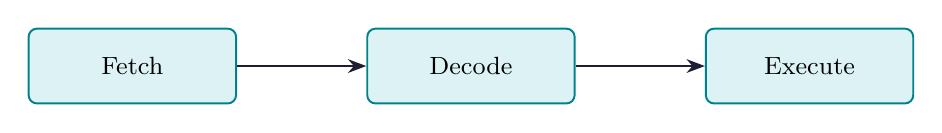
\begin{tikzpicture}
\node[block] (f) at (0,0) {Fetch};
\node[block] (d) at (4.3,0) {Decode};
\node[block] (e) at (8.6,0) {Execute};
\draw[arrow] (f) -- (d);
\draw[arrow] (d) -- (e);
\end{tikzpicture}
\end{tcolorbox}
\begin{tcolorbox}[examplebox,title={Ideal Pipeline Timing}]
For $N$ instructions in a $k$-stage pipeline with equal stage time $t_c$ and no stalls, the first result needs $k$ clocks and the remaining $N-1$ results need one clock each.
\[
 T_{\mathrm{pipe}}=(k+N-1)t_c.
\]
For $k=3$, $N=8$ and $t_c=10$ ns, the ideal time is 100 ns. Executing each full instruction before starting the next takes $Nk t_c=240$ ns under the same stage-time model. The ideal speedup for this short sequence is 2.4.
\end{tcolorbox}

\section{Arm Cores and Microcontroller Organisation}
\begin{tcolorbox}[defbox,title={Arm Core and Microcontroller}]
An \textbf{Arm core} executes the instruction set for a given Arm architecture. A microcontroller integrates that core with Flash, SRAM, clock and reset logic, GPIO and other peripheral blocks. Peripheral register names and pin mappings depend on the chip.
\end{tcolorbox}
\subsection{ARM7TDMI and Cortex-M3}
ARM7TDMI implements Armv4T, with a three-stage pipeline, 32-bit ARM instructions and compact 16-bit Thumb instructions. It has separate fast interrupt and ordinary interrupt (FIQ and IRQ) exception paths with banked state for exception modes. Cortex-M3 implements Armv7-M and executes Thumb instructions, including 16- and 32-bit encodings. It integrates the Nested Vectored Interrupt Controller (NVIC) and uses a different exception model. Cortex-A generally targets application processors, Cortex-R targets timing-critical systems and Cortex-M targets microcontrollers.
\subsection{Registers and Load/Store Example}
On Cortex-M3, R0--R12 are general-purpose registers, R13 denotes SP, R14 is the link register (LR), and R15 denotes PC. The program status is available through xPSR. On reset, the first vector-table word initializes the main stack pointer and the next word gives the reset handler entry. For a call, BL saves the return link and branches. The following Thumb sequence adds two words, assuming R0 points to aligned inputs and R3 points to writable word storage.
\begin{verbatim}
        LDR  r1,[r0,#0]
        LDR  r2,[r0,#4]
        ADDS r1,r1,r2       ; C records unsigned carry
        STR  r1,[r3,#0]
\end{verbatim}

\par\ifdim\dimexpr\pagegoal-\pagetotal\relax<105pt\relax\newpage\fi
\section{ARM Microcontroller Interface Design}
\begin{tcolorbox}[defbox,title={Memory-Mapped I/O}]
\textbf{Memory-mapped I/O} gives a peripheral register an address in the processor's address map. The CPU uses ordinary load and store instructions to reach that register. Firmware must use the supported width and register semantics, and enable the peripheral clock where required.
\end{tcolorbox}
\begin{tcolorbox}[tikzbox,title={Microcontroller Interface Paths}]
\centering
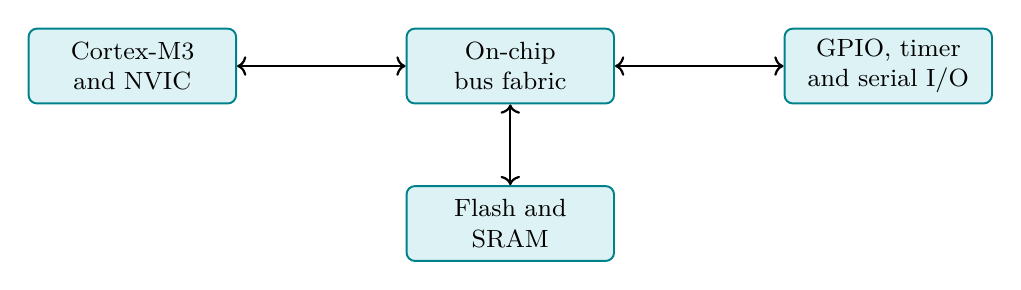
\begin{tikzpicture}
\node[block] (core) at (0,0) {Cortex-M3\\and NVIC};
\node[block] (bus) at (4.8,0) {On-chip\\bus fabric};
\node[block] (per) at (9.6,0) {GPIO, timer\\and serial I/O};
\node[block] (mem) at (4.8,-2) {Flash and SRAM};
\draw[<->,thick] (core) -- (bus);
\draw[<->,thick] (bus) -- (per);
\draw[<->,thick] (bus) -- (mem);
\end{tikzpicture}
\end{tcolorbox}
\subsection{Design Checklist}
\begin{enumerate}[leftmargin=*,itemsep=4pt]
\item \textbf{Choose an interface.} Determine signal rate, direction, voltage, device count and timing. GPIO suits discrete signals. A timer produces independent periodic events. Select a serial interface for a continuous data stream.
\item \textbf{Make the connections.} Use a common reference ground, suitable supply decoupling and levels compatible with the MCU and device. Use pull-ups where required. Use a transistor or driver for loads beyond the pin rating.
\item \textbf{Configure the MCU.} Enable peripheral clocks and select pin mode or alternate function. Set timing, data format and polarity. Clear stale status before enabling requests.
\item \textbf{Select a transfer method.} Poll for simple tests, use interrupts for asynchronous events, or use DMA for repeated transfers when the hardware supports it.
\item \textbf{Test failure cases.} Check reset states, clock assumptions, timeouts, busy flags, missed interrupts, overrun and disconnected devices.
\end{enumerate}

\subsection{GPIO and External Interrupt on STM32F103}
The register examples use STM32F103 with default pin mapping. Verify that the chosen package exposes the pins. For an active-high LED on PA5, connect PA5 through a current-limiting resistor to the LED anode and return its cathode to ground. For an active-low switch on PA0, use an internal or external pull-up and connect the switch to ground.
\begin{tcolorbox}[examplebox,title={LED and Push-Button Interface}, title after break={LED and Push-Button Interface (contd.)}]
\begin{enumerate}[leftmargin=*,itemsep=4pt]
\item Enable GPIOA in \texttt{RCC\_APB2ENR}. For interrupt pin routing also enable the alternate-function I/O (AFIO) clock.
\item Configure PA5 as general-purpose push-pull output at 2 MHz using its four-bit field in \texttt{GPIOA\_CRL}: CNF=00 and MODE=10. Write bit 5 of \texttt{GPIOA\_BSRR} to set PA5 or bit 21 to clear it.
\item Configure PA0 as input with pull-up/pull-down (CNF=10, MODE=00), then set ODR bit 0 to select the pull-up. Read bit 0 of \texttt{GPIOA\_IDR} for polling.
\item For an interrupt, route port A to EXTI0 in AFIO, select a falling edge and unmask EXTI0. Clear pending by writing 1 to EXTI PR bit 0, then enable EXTI0 in the NVIC. In the handler, acknowledge the event through the peripheral and debounce the switch.
\end{enumerate}
For a 3.3 V supply, a 2.0 V LED drop and 4 mA target, $R\approx(3.3-2.0)/0.004=325\ \Omega$. A $330\ \Omega$ resistor gives approximately 3.9 mA under the stated assumptions. Confirm the pin current and output-voltage limits in the device data sheet.
\end{tcolorbox}

\subsection{Serial Interfaces and Timer Output}
\par\addvspace{5pt}
\begingroup
\setlength{\extrarowheight}{2.5pt}
\noindent\begin{tabularx}{\linewidth}{|B{2.4cm}|Y|Y|}
\hline
\textbf{Interface} & \textbf{Signals and operation} & \textbf{Design decision} \\ \hline
UART & TX, RX and common ground. Asynchronous framed data. & Match baud and frame format. Cross logic-level TX and RX between devices. Use a line transceiver when required. \\ \hline
SPI & SCK, controller output and input, and a device-select signal. Synchronous transfer. & Match clock polarity and phase, transfer order and chip-select timing. Keep only the intended device selected. \\ \hline
I2C & SDA and SCL with open-drain outputs and pull-ups. Addressed transfers and ACK. & Choose pull-ups and rate for the bus capacitance. Ensure the addresses and signal levels are compatible. \\ \hline
Timer/PWM & A timer counts clock ticks and drives an output compare channel. & Select the clock, divider, period and compare value. Configure the output pin's alternate function. \\ \hline
\end{tabularx}\par
\endgroup
For USART1 on STM32F103 with default mapping, PA9 is TX and PA10 is RX. Enable the USART and GPIO clocks, configure alternate-function push-pull TX and an appropriate input mode for RX, set baud and frame format, then enable transmit and receive. For an oversampling-by-16 USART at a 72 MHz peripheral clock and 9600 baud, the divisor in the baud-rate register encoding is $72000000/9600=7500$, or \texttt{1D4CH}. Use the actual peripheral clock rather than assuming it equals the CPU frequency.
\begin{tcolorbox}[examplebox,title={Generate 1 kHz PWM at 25 Percent Duty}]
For edge-aligned upcounting with PWM mode 1 and active-high output, take the timer input clock as 72 MHz, the prescaler as 71 and the auto-reload register as 999:
\begin{align*}
 f_{\mathrm{count}} &= 72\,\mathrm{MHz}/(71+1)=1\,\mathrm{MHz},\\
 f_{\mathrm{PWM}} &= 1\,\mathrm{MHz}/(999+1)=1\,\mathrm{kHz},\\
 \mathrm{CCR} &= 0.25(999+1)=250.
\end{align*}
The output is active for the first 250 of the 1000 counts. On STM32F103, an APB prescaler can change the relationship between the peripheral-bus clock and timer clock, so check the clock tree before using these values.
\end{tcolorbox}
\par\addvspace{7pt}\noindent
ADC pins use analog mode, a legal analog input range and the expected reference. Sampling time must suit source impedance. A sensor application can use a timer trigger and DMA, where supported, to record samples while the CPU performs other work.

\subsection{Worked System Design: Periodic SPI Sensor Reading}
\begin{tcolorbox}[examplebox,title={Wire, Configure, Transfer and Verify}]
Assume a 3.3 V SPI sensor and an STM32F103 using default SPI1 routing.
\begin{enumerate}[leftmargin=*,itemsep=4pt]
\item Connect PA5 to the sensor clock, PA7 to its data input, PA6 to its data output, and a GPIO such as PA4 to chip select. Use a common ground. Check voltage limits and keep chip select inactive while the MCU starts.
\item Enable the GPIO and SPI1 clocks. Set SCK and MOSI to alternate-function output, MISO as input and PA4 as a GPIO output. Set the master clock divider, bit order, polarity and phase from the sensor specification.
\item For each sample, assert chip select, transmit the read command, and clock the response bytes while sending appropriate filler bytes. Read the receive register as data becomes available. Finish the transfer before releasing chip select.
\item Use a hardware timer to schedule samples. Use a timeout so a failed or missing device does not hold the application in a busy loop. Verify clock, chip-select timing and data order on a logic analyser.
\end{enumerate}
SPI is full duplex at the wire level. Reading a response requires transmitted clocks, even when the outgoing data bits have no meaning for that phase of the transaction.
\end{tcolorbox}

\subsection*{References}
Arm's \href{https://support.arm.com/documentation/ddi0210/c/Introduction/About-the-ARM7TDMI-core}{ARM7TDMI technical reference} and \href{https://documentation-service.arm.com/static/5ea823e69931941038df1af5}{Cortex-M3 Devices Generic User Guide} explain the core features. STMicroelectronics \href{https://www.st.com/resource/en/reference_manual/rm0008-.pdf}{RM0008} describes the STM32F103 register and peripheral examples.

\newpage
\begin{center}
{\large\bfseries\color{myred} Quick Revision --- Module 4}\\[3pt]
{\small\color{mydark} RISC Processors and ARM Interfacing $|$ EC403}
\end{center}
\noindent{\color{myred}\rule{\linewidth}{1.2pt}}\vspace{4pt}
\begin{tcolorbox}[formulabox,title={Key Formulas at a Glance}]
\renewcommand{\arraystretch}{1.35}
\noindent\begin{tabularx}{\linewidth}{B{4.2cm}Y}
Ideal pipeline time & $(k+N-1)t_c$ for $k$ stages and $N$ instructions. \\
Timer count clock & $f_{\mathrm{TIM}}/(\mathrm{PSC}+1)$. \\
Edge-aligned PWM & $f_{\mathrm{count}}/(\mathrm{ARR}+1)$. Duty $=\mathrm{CCR}/(\mathrm{ARR}+1)$ under the stated PWM model. \\
LED resistor & $R\approx(V_{\mathrm{out}}-V_F)/I$. \\
\end{tabularx}\par
\end{tcolorbox}
\begin{tcolorbox}[defbox,title={One-Line Definitions}]
\begin{itemize}[leftmargin=*,itemsep=3pt]
\item \textbf{Load/store architecture:} Arithmetic mainly uses registers and explicit loads and stores access memory.
\item \textbf{NVIC:} Cortex-M controller that prioritises and dispatches supported interrupts.
\item \textbf{Alternate function:} A pin mode that connects a peripheral signal to a physical pin.
\item \textbf{PWM duty cycle:} Fraction of each period during which the output is active.
\end{itemize}
\end{tcolorbox}
\begin{tcolorbox}[exambox,title={Frequently Asked / Viva Questions}]
\begin{enumerate}[leftmargin=*,label=\textbf{Q\arabic*.},itemsep=5pt]
\item \Q{What separates a load from a store?} A load moves a value from memory into a register, and a store moves a register value to memory.
\item \Q{What does a pipeline improve?} Instruction throughput by overlapping stages.
\item \Q{Which instruction states does ARM7TDMI support?} ARM and Thumb.
\item \Q{Does Cortex-M3 execute ARM-state instructions?} Cortex-M3 executes Thumb instructions.
\item \Q{What is a peripheral clock gate?} A control that enables or stops the clock to a peripheral block.
\item \Q{Why is a pull-up used on an active-low switch input?} It provides a defined high level when the switch is open.
\item \Q{What advantage does BSRR give on STM32F103?} It sets or resets selected output latch bits without a read-modify-write of ODR.
\item \Q{Why use a hardware timer to generate PWM?} The waveform timing does not depend on software delays.
\item \Q{Which serial bus typically uses open-drain pins and pull-ups?} I2C.
\item \Q{What must SPI devices agree on?} Clock polarity, phase, bit order and device-select timing.
\item \Q{Where do you find register and pin details?} Use the MCU reference manual and the data sheet for the selected part and package.
\end{enumerate}
\end{tcolorbox}
\begin{tcolorbox}[tikzbox,title={Choose an Interface at a Glance}]
\par\addvspace{5pt}
\begingroup
\setlength{\extrarowheight}{2.5pt}
\noindent\begin{tabularx}{\linewidth}{|B{3.2cm}|Y|Y|}
\hline
\textbf{Task} & \textbf{Interface} & \textbf{Design check} \\ \hline
Read a switch & GPIO with pull-up & Input level, edge and debounce. \\ \hline
Send periodic pulses & Timer output & Clock tree, period and duty cycle. \\ \hline
Exchange serial data & UART, SPI or I2C & Format, wiring, logic levels and timing. \\ \hline
\end{tabularx}\par
\endgroup
\end{tcolorbox}


\end{document}
